\documentclass[12pt,a4paper]{article}

\usepackage[utf8]{inputenc}
\usepackage[UKenglish]{babel}
\usepackage[a4paper,left=20mm,right=20mm,top=20mm,bottom=20mm,headheight=15pt]{geometry}
\usepackage{mathptmx}
\usepackage{amsmath,amssymb}
\usepackage{booktabs}
\usepackage{graphicx}
\usepackage{listings}
\usepackage{fancyhdr}
\usepackage{float}
\usepackage{xurl}
\usepackage{hyperref}

\hypersetup{
    colorlinks=true,
    linkcolor=black,
    filecolor=black,
    urlcolor=blue,
    citecolor=black
}

\lstset{
    basicstyle=\fontsize{7.5pt}{9.2pt}\ttfamily,
    breaklines=true,
    breakatwhitespace=true,
    showstringspaces=false,
    frame=none,
    numbers=none,
    captionpos=b,
    aboveskip=0.4em,
    belowskip=0.4em
}

\pagestyle{fancy}
\fancyhf{}
\fancyhead[L]{\small Cryptography and Security}
\fancyhead[R]{\small Laboratory Work No. 2}
\fancyfoot[C]{\thepage}
\renewcommand{\headrulewidth}{0.4pt}

\begin{document}

% ---------------------------------------------------------
% TITLE PAGE
% ---------------------------------------------------------
\begin{titlepage}
    \centering
    {\bfseries\large MINISTRY OF EDUCATION AND RESEARCH\\
    OF THE REPUBLIC OF MOLDOVA\par}
    \vspace{0.4cm}
    {\bfseries Technical University of Moldova\par}
    \vspace{0.2cm}
    {\bfseries Faculty of Computers, Informatics and Microelectronics\par}
    \vspace{0.2cm}
    {\bfseries Department of Software Engineering and Automation\par}
    
    \vspace{3.5cm}
    
    {\Large\bfseries Ilie Covali, FAF-243\par}
    
    \vspace{1.5cm}
    
    {\huge\bfseries Report\par}
    \vspace{0.3cm}
    {\Large\bfseries Laboratory Work No. 2\par}
    \vspace{0.2cm}
    {\large Cryptography and Security\par}
    \vspace{0.4cm}
    {\large\textbf{Topic:} Cryptanalysis of Monoalphabetic Ciphers\par}
    \vspace{0.2cm}
    {\large Frequency Analysis of Variant 9\par}
    
    \vfill
    
    \begin{flushleft}
    \large
    \textbf{Checked by:}\\
    Maia Zaica, university assistant
    \end{flushleft}
    
    \vspace{1cm}
    
    {\large Chi\c{s}in\u{a}u -- 2026\par}
\end{titlepage}

\pagenumbering{arabic}
\setcounter{page}{2}

\tableofcontents
\newpage

% ---------------------------------------------------------
% INTRODUCTION
% ---------------------------------------------------------
\section*{INTRODUCTION}
\addcontentsline{toc}{section}{Introduction}
The purpose of this laboratory work is to recover an English plaintext encrypted with a monoalphabetic substitution cipher. I solved Variant 9 manually with the frequency-analysis service specified in the laboratory handout (\url{https://crypto.interactive-maths.com/frequency-analysis-breaking-the-code.html}). The attack combines letter frequencies with repeated patterns, common short words, and contextual recognition.

At every stage below, confirmed plaintext letters are shown in lowercase while unresolved ciphertext symbols remain uppercase. This makes the progress of the attack visible and reproduces the notation used by the online tool. The complete text is included after every iteration, as required by the worked-example format in the handout.

\newpage

% ---------------------------------------------------------
% 1 SHORT THEORY
% ---------------------------------------------------------
\section{Short Theory}
\subsection{Monoalphabetic Substitution}
In a monoalphabetic substitution cipher, every plaintext letter is replaced by one fixed ciphertext letter. The key is therefore a permutation of the alphabet. For plaintext letter $x$ and substitution permutation $\pi$, encryption and decryption can be written as
\begin{equation}
y = \pi(x), \qquad x = \pi^{-1}(y).
\end{equation}
Spaces, punctuation, and digits are not encrypted in this task. Although there are $26! \approx 4.03 \times 10^{26}$ possible alphabet permutations, the cipher preserves the statistical structure of the language: a frequent plaintext letter still produces a frequent ciphertext symbol, repeated letters remain repeated, and identical word patterns remain visible.

\subsection{Frequency and Pattern Analysis}
English text has a characteristic distribution in which \texttt{e}, \texttt{t}, \texttt{a}, \texttt{o}, \texttt{i}, and \texttt{n} are among the most common letters. Frequency comparison provides hypotheses, but it is not sufficient by itself because a finite passage differs from the ideal distribution. The hypotheses must be checked against common digraphs such as \texttt{th} and \texttt{he}, common trigraphs such as \texttt{the} and \texttt{and}, one-letter words, word lengths, repeated-letter patterns, and the meaning of the surrounding sentence.

The practical attack is iterative. A plausible substitution is entered, the entire text is updated, and newly visible word fragments provide evidence for the next substitution. Incorrect hypotheses can be reversed; a correct hypothesis normally completes several patterns at once.

\newpage

% ---------------------------------------------------------
% 2 FREQUENCY ANALYSIS OF VARIANT 9
% ---------------------------------------------------------
\section{Frequency Analysis of Variant 9}
\subsection{Initial Intercept}
The intercepted ciphertext supplied for Variant 9 is shown below. The line wrapping is only for readability and does not change the message. Reading convention: CAPITALS are unresolved ciphertext symbols; lowercase letters are confirmed plaintext substitutions.

\begin{lstlisting}[caption={Variant 9 intercepted ciphertext}, label={lst:intercept}]
VTHQ GVR PVWWXGJ NC TSAVIWX'P OXPL AINDJQW XGWN USTF T GVR HXUQVITSUQTAVW, XG
RQXHQ ANWQ WQV USTXGWVYW TGO WQV HXUQVIWVYW VBDXKTSVGWP TIVHQTGJVO XG IVJTIO WN
NGV TGNWQVI. WQVIV TIV TP ZTGF NC WQVPV TSUQTAVWPTP WQVIV TIV UNPXWXNGP NC QXP
OXPL, TGO WQXP ZDSWXUSXHXWF ZVTGP WQTW TSAVIWXQVIV OVKXPVO WQV CXIPW
UNSFTSUQTAVWXH HXUQVI.WQXP THQXVKVZVGW--HIXWXHTS XG WQV QXPWNIF NC HIFUWNSNJF
--TSAVIWX WQVGTONIGVO AF TGNWQVI IVZTILTASV XGKVGWXNG: VGHXUQVIVO HNOV. XW RTP
CNIWQXP WQTW QV QTO UDW GDZAVIP XG WQV NDWVI IXGJ. XG T WTASV QV UVIZDWVOWQV
GDZAVIP 1 WN 4 XG WRN-, WQIVV-, TGO CNDI-OXJXW JINDUP, CINZ 11 WN4444, TGO DPVO
WQVPV TP 336 HNOVJINDUP CNI T PZTSS HNOV. "XG WQXP WTASV,THHNIOXGJ WN TJIVVZVGW,
RV PQTSS VGWVI XG WQV KTIXNDP SXGVP TW WQVGDZAVIP RQTWVKVI HNZUSVWV UQITPVP RV
USVTPV, CNI VYTZUSV,HNIIVPUNGOXGJ WN 12, 'RV QTKV ZTOV IVTOF WQV PQXUP RQXHQ RV
UINZXPVOTGO PDUUSXVO WQVZ RXWQ WINNUP TGO JITXG.' " WQVPV HNOV KTSDVP OXO
GNWHQTGJV, TGF ZNIV WQTG WQV ZXYVO TSUQTAVW NC WQV OXPL OXO. ADW WQV
OXJXWPIVPDSWXGJ CINZ TG VGHNOXGJ RVIV WQVG VGHXUQVIVO RXWQ WQV OXPL EDPW TP XCWQVF
RVIV USTXGWVYW SVWWVIP. XG TSAVIWX'P RNIOP, "WQVPV GDZAVIP X WQVGXGPVIW XG ZF
ZVPPTJV THHNIOXGJ WN WQV CNIZDST NC WQV HXUQVI, IVUIVPVGWXGJWQVZ AF WQV SVWWVIP
WQTW OVGNWV WQVPV GDZAVIP." WQVPV GDZAVIP WQDPHQTGJVO WQVXI HXUQVIWVYW VBDXKTSVGWP
TP WQV OXPL WDIGVO. QVGHV 341,UVIQTUP ZVTGXGJ "UNUV," ZXJQW AVHNZV ZIU TW NGV
UNPXWXNG TGO CHN TWTGNWQVI. WQXP HNGPWXWDWVP TG VYHVSSVGW CNIZ NC VGHXUQVIVO HNOV,
TGO EDPWQNR UIVHNHXNDP TSAVIWX RTP ZTF AV PVVG AF WQV CTHW WQTW WQV ZTENIUNRVIP NC
WQV VTIWQ OXO GNW AVJXG WN VGHXUQVI WQVXI HNOV ZVPPTJVP DGWXS400 FVTIP STWVI, GVTI
WQV VGO NC WQV 19WQ HVGWDIF, TGO VKVG WQVG WQVXIPFPWVZP RVIV ZDHQ PXZUSVI WQTG
WQXP.TSAVIWX'P WQIVV IVZTILTASV CXIPWP--WQV VTISXVPW RVPWVIG VYUNPXWXNG
NCHIFUWTGTSFPXP, WQV XGKVGWXNG NC UNSFTSUQTAVWXV PDAPWXWDWXNG, TGO WQVXGKVGWXNG NC
VGHXUQVIVO HNOV--ZTLV QXZ WQV CTWQVI NC RVPWVIGHIFUWNSNJF. ADW TSWQNDJQ QXP
WIVTWXPV RTP UDASXPQVO XG XWTSXTG XG THNSSVHWXNG NC QXP RNILP XG 1568, TGO
TSWQNDJQ QXP XOVTP RVIV TAPNIAVO AFUTUTS HIFUWNSNJXPWP TGO UVIQTUP XGCSDVGHVO WQV
PHXVGHV'P OVKVSNUZVGW,WQVF GVKVI QTO WQV OFGTZXH XZUTHW WQTW PDHQ
UINOXJXNDPTHHNZUSXPQZVGWP NDJQW WN QTKV UINODHVO. PFZNGOP' VKTSDTWXNG NC QXPRNIL
XG JVGVITS ZTF ANWQ VYUSTXG RQF TGO PDZZTIXMV WQV ZNOVIG KXVR NC QXP HIFUWNSNJXHTS
HNGWIXADWXNGP:"WQXP ZTG NC ZTGF-PXOVO JVGXDP HTZV XGWN WQV RNISO WNN PNNG CNI
WQVUVICVHW VYVIHXPV NC QXP PXGJDSTI CTHDSWXVP. RQVWQVI RV IVJTIO QXZ CINZ WQVUNXGW
NC KXVR NC TIW, NC PHXVGHV, NI NC SXWVITWDIV, QV NHHDUXVP XG VTHQOVUTIWZVGW WQV
UNPXWXNG NC UIVHDIPNI, UXNGVVI, TGO XGOXHTWNI. TSRTFPNIXJXGTS TGO TSRTFP CVIWXSV,
QV UINUQVPXVO NC STGOP QV RTP GNW UIXKXSVJVOWN VGWVI, SVTKXGJ WQV ZVZNIF NC OXZ
TGO KTIXVO JIVTWGVPP ITWQVI WQTG TGFPNSXO ZNGDZVGW AVQXGO QXZ."UNSFTSUQTAVWXHXWF
WNNL TGNWQVI PWVU CNIRTIO XG 1518, RXWQ WQVTUUVTITGHV NC WQV CXIPW UIXGWVO ANNL NG
HIFUWNSNJF, RIXWWVG AF NGV NC WQVZNPW CTZNDP XGWVSSVHWDTSP NC QXP OTF. WQXP RTP
ENQTGGVP WIXWQVZXDP, TAVGVOXHWXGV ZNGL RQNPV OTAASXGJ XG TSHQVZF TGO NWQVI ZFPWXH
UNRVIPZTOV QXZ NGV NC WQV ZNPW IVKVIVO CXJDIVP XG NHHDSW PHXVGHV, RQXSV QXPZNIV
PNSXO PHQNSTIPQXU RNG QXZ WQV WXWSV NC "CTWQVI NC AXAXSXNJITUQF." XG1518, T FVTI
TGO T QTSC TCWVI QXP OVTWQ, QXP UNSFJITUQXTV SXAIX PVY, SNTGGXPWIXWQVZXX TAATWXP
UVTUNSXWTGX, BDNGOTZ PUTGQVXZVGPXP, TO ZTYXZXSXTGDZHTVPTIVZ ("PXY ANNLP NC
UNSFJITUQF, AF ENQTGGVP WIXWQVZXDP, TAANW TWRDIMADIJ, CNIZVISF TW PUTGQVXZ, CNI
WQV VZUVINI ZTYXZXSXTG") RTPUDASXPQVO. AF CTI WQV ADSL NC WQV KNSDZV HNGPXPWP NC
WQV HNSDZGP NCRNIOP UIXGWVO XG STIJV JNWQXH WFUV WQTW WIXWQVZXDP DPVO XG QXP
PFPWVZP NCHIFUWNJITUQF. ADW XG WQV RNIL'P ANNL K TUUVTIP, CNI WQV CXIPW WXZV,
WQVPBDTIV WTASV, NI WTASVTD. WQXP XP WQV VSVZVGWTS CNIZ NC
UNSFTSUQTAVWXHPDAPWXWDWXNG, CNI XW VYQXAXWP TSS TW NGHV TSS WQV HXUQVI TSUQTAVWP
XG TUTIWXHDSTI PFPWVZ. WQVPV TIV DPDTSSF TSS WQV PTZV PVBDVGHV NC SVWWVIP,
ADWPQXCWVO WN OXCCVIVGW UNPXWXNGP XG IVSTWXNG WN WQV USTXGWVYW TSUQTAVW, TP
XGTSAVIWX'P OXPL WQV XGGVI TSUQTAVW TPPDZVO OXCCVIVGW UNPXWXNGP XG IVJTIO WNWQV
NDWVI TSUQTAVW. WQV WTASVTD PVWP WQVZ NDW XG NIOVISF CTPQXNG--WQVTSUQTAVWP NC WQV
PDHHVPPXKV UNPXWXNGP STXO NDW XG INRP NGV AVSNR WQVNWQVI, VTHQ TSUQTAVW PQXCWVO
NGV USTHV WN WQV SVCW NC WQV NGV TANKV. VTHQINR WQDP NCCVIP T OXCCVIVGW PVW NC
HXUQVI PDAPWXWDWVP WN WQV SVWWVIP NC WQVUSTXGWVYW TSUQTAVW TW WQV WNU. PXGHV WQVIV
HTG AV NGSF TP ZTGF INRP TPWQVIV TIV SVWWVIP XG WQV TSUQTAVW, WQV WTASVTD XP
PBDTIV.WQV PXZUSVPW WTASVTD XP NGV WQTW DPVP WQV GNIZTS TSUQTAVW XG
KTIXNDPUNPXWXNGP TP WQV HXUQVI TSUQTAVWP. VTHQ HXUQVI TSUQTAVW UINODHVP, XGNWQVI
RNIOP, T HTVPTI PDAPWXWDWXNG.
\end{lstlisting}

\newpage
\subsection{Observed Frequencies}
I selected Find Frequencies on the specified website. The image compares the standard English distribution with the frequencies of this intercept. The most frequent ciphertext letters are V with 496 occurrences (13.1\%), W with 378 (9.9\%), T and X with 293 (7.7\% each), N with 257 (6.8\%), P with 256 (6.7\%), Q with 251 (6.6\%), and G and I with 232 (6.1\% each).

\begin{figure}[H]
    \centering
    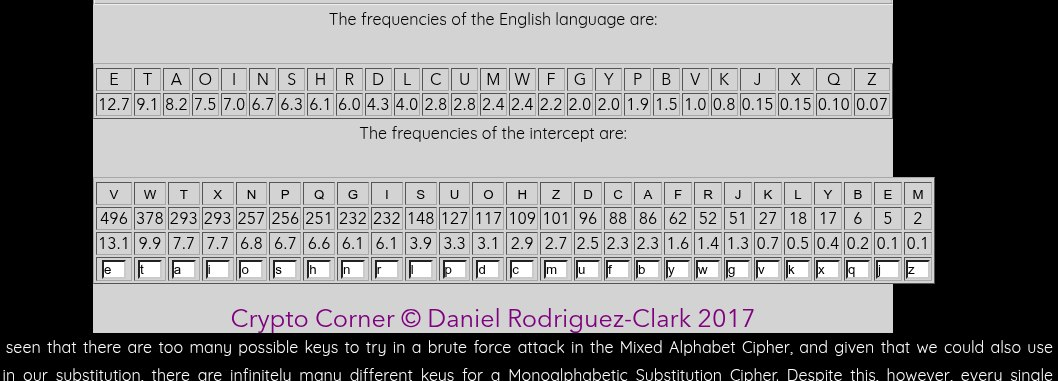
\includegraphics[width=\textwidth]{images/frequencies_tool.png}
    \caption{Reference English frequencies, Variant 9 frequencies, and the completed substitutions}
    \label{fig:frequencies}
\end{figure}

The high counts provide starting hypotheses, while the words created after each replacement decide whether those hypotheses are credible.

\vspace{0.8em}

% ---------------------------------------------------------
% 3 ITERATIVE DECODING PROCESS
% ---------------------------------------------------------
\section{Iterative Decoding Process}
Each state below is cumulative. A letter changes to lowercase only in the iteration where its substitution is accepted; every still-undiscovered symbol remains uppercase.
Reading convention: CAPITALS are unresolved ciphertext symbols; lowercase letters are confirmed plaintext substitutions.

\clearpage
\subsection{Iteration 1}
\textbf{New substitutions:} V$\to$e.

\textbf{Reasoning.} The frequency tool showed that V is the most common ciphertext letter: 496 occurrences, or 13.1% of the intercept. Since e is the most frequent English letter (12.7% reference frequency), I first tested V as e.

\begin{lstlisting}[caption={Complete text after iteration 1}, label={lst:iter1}]
eTHQ GeR PeWWXGJ NC TSAeIWX'P OXPL AINDJQW XGWN USTF T GeR HXUQeITSUQTAeW, XG
RQXHQ ANWQ WQe USTXGWeYW TGO WQe HXUQeIWeYW eBDXKTSeGWP TIeHQTGJeO XG IeJTIO WN
NGe TGNWQeI. WQeIe TIe TP ZTGF NC WQePe TSUQTAeWPTP WQeIe TIe UNPXWXNGP NC QXP
OXPL, TGO WQXP ZDSWXUSXHXWF ZeTGP WQTW TSAeIWXQeIe OeKXPeO WQe CXIPW
UNSFTSUQTAeWXH HXUQeI.WQXP THQXeKeZeGW--HIXWXHTS XG WQe QXPWNIF NC HIFUWNSNJF
--TSAeIWX WQeGTONIGeO AF TGNWQeI IeZTILTASe XGKeGWXNG: eGHXUQeIeO HNOe. XW RTP
CNIWQXP WQTW Qe QTO UDW GDZAeIP XG WQe NDWeI IXGJ. XG T WTASe Qe UeIZDWeOWQe
GDZAeIP 1 WN 4 XG WRN-, WQIee-, TGO CNDI-OXJXW JINDUP, CINZ 11 WN4444, TGO DPeO
WQePe TP 336 HNOeJINDUP CNI T PZTSS HNOe. "XG WQXP WTASe,THHNIOXGJ WN TJIeeZeGW,
Re PQTSS eGWeI XG WQe KTIXNDP SXGeP TW WQeGDZAeIP RQTWeKeI HNZUSeWe UQITPeP Re
USeTPe, CNI eYTZUSe,HNIIePUNGOXGJ WN 12, 'Re QTKe ZTOe IeTOF WQe PQXUP RQXHQ Re
UINZXPeOTGO PDUUSXeO WQeZ RXWQ WINNUP TGO JITXG.' " WQePe HNOe KTSDeP OXO
GNWHQTGJe, TGF ZNIe WQTG WQe ZXYeO TSUQTAeW NC WQe OXPL OXO. ADW WQe
OXJXWPIePDSWXGJ CINZ TG eGHNOXGJ ReIe WQeG eGHXUQeIeO RXWQ WQe OXPL EDPW TP XCWQeF
ReIe USTXGWeYW SeWWeIP. XG TSAeIWX'P RNIOP, "WQePe GDZAeIP X WQeGXGPeIW XG ZF
ZePPTJe THHNIOXGJ WN WQe CNIZDST NC WQe HXUQeI, IeUIePeGWXGJWQeZ AF WQe SeWWeIP
WQTW OeGNWe WQePe GDZAeIP." WQePe GDZAeIP WQDPHQTGJeO WQeXI HXUQeIWeYW eBDXKTSeGWP
TP WQe OXPL WDIGeO. QeGHe 341,UeIQTUP ZeTGXGJ "UNUe," ZXJQW AeHNZe ZIU TW NGe
UNPXWXNG TGO CHN TWTGNWQeI. WQXP HNGPWXWDWeP TG eYHeSSeGW CNIZ NC eGHXUQeIeO HNOe,
TGO EDPWQNR UIeHNHXNDP TSAeIWX RTP ZTF Ae PeeG AF WQe CTHW WQTW WQe ZTENIUNReIP NC
WQe eTIWQ OXO GNW AeJXG WN eGHXUQeI WQeXI HNOe ZePPTJeP DGWXS400 FeTIP STWeI, GeTI
WQe eGO NC WQe 19WQ HeGWDIF, TGO eKeG WQeG WQeXIPFPWeZP ReIe ZDHQ PXZUSeI WQTG
WQXP.TSAeIWX'P WQIee IeZTILTASe CXIPWP--WQe eTISXePW RePWeIG eYUNPXWXNG
NCHIFUWTGTSFPXP, WQe XGKeGWXNG NC UNSFTSUQTAeWXe PDAPWXWDWXNG, TGO WQeXGKeGWXNG NC
eGHXUQeIeO HNOe--ZTLe QXZ WQe CTWQeI NC RePWeIGHIFUWNSNJF. ADW TSWQNDJQ QXP
WIeTWXPe RTP UDASXPQeO XG XWTSXTG XG THNSSeHWXNG NC QXP RNILP XG 1568, TGO
TSWQNDJQ QXP XOeTP ReIe TAPNIAeO AFUTUTS HIFUWNSNJXPWP TGO UeIQTUP XGCSDeGHeO WQe
PHXeGHe'P OeKeSNUZeGW,WQeF GeKeI QTO WQe OFGTZXH XZUTHW WQTW PDHQ
UINOXJXNDPTHHNZUSXPQZeGWP NDJQW WN QTKe UINODHeO. PFZNGOP' eKTSDTWXNG NC QXPRNIL
XG JeGeITS ZTF ANWQ eYUSTXG RQF TGO PDZZTIXMe WQe ZNOeIG KXeR NC QXP HIFUWNSNJXHTS
HNGWIXADWXNGP:"WQXP ZTG NC ZTGF-PXOeO JeGXDP HTZe XGWN WQe RNISO WNN PNNG CNI
WQeUeICeHW eYeIHXPe NC QXP PXGJDSTI CTHDSWXeP. RQeWQeI Re IeJTIO QXZ CINZ WQeUNXGW
NC KXeR NC TIW, NC PHXeGHe, NI NC SXWeITWDIe, Qe NHHDUXeP XG eTHQOeUTIWZeGW WQe
UNPXWXNG NC UIeHDIPNI, UXNGeeI, TGO XGOXHTWNI. TSRTFPNIXJXGTS TGO TSRTFP CeIWXSe,
Qe UINUQePXeO NC STGOP Qe RTP GNW UIXKXSeJeOWN eGWeI, SeTKXGJ WQe ZeZNIF NC OXZ
TGO KTIXeO JIeTWGePP ITWQeI WQTG TGFPNSXO ZNGDZeGW AeQXGO QXZ."UNSFTSUQTAeWXHXWF
WNNL TGNWQeI PWeU CNIRTIO XG 1518, RXWQ WQeTUUeTITGHe NC WQe CXIPW UIXGWeO ANNL NG
HIFUWNSNJF, RIXWWeG AF NGe NC WQeZNPW CTZNDP XGWeSSeHWDTSP NC QXP OTF. WQXP RTP
ENQTGGeP WIXWQeZXDP, TAeGeOXHWXGe ZNGL RQNPe OTAASXGJ XG TSHQeZF TGO NWQeI ZFPWXH
UNReIPZTOe QXZ NGe NC WQe ZNPW IeKeIeO CXJDIeP XG NHHDSW PHXeGHe, RQXSe QXPZNIe
PNSXO PHQNSTIPQXU RNG QXZ WQe WXWSe NC "CTWQeI NC AXAXSXNJITUQF." XG1518, T FeTI
TGO T QTSC TCWeI QXP OeTWQ, QXP UNSFJITUQXTe SXAIX PeY, SNTGGXPWIXWQeZXX TAATWXP
UeTUNSXWTGX, BDNGOTZ PUTGQeXZeGPXP, TO ZTYXZXSXTGDZHTePTIeZ ("PXY ANNLP NC
UNSFJITUQF, AF ENQTGGeP WIXWQeZXDP, TAANW TWRDIMADIJ, CNIZeISF TW PUTGQeXZ, CNI
WQe eZUeINI ZTYXZXSXTG") RTPUDASXPQeO. AF CTI WQe ADSL NC WQe KNSDZe HNGPXPWP NC
WQe HNSDZGP NCRNIOP UIXGWeO XG STIJe JNWQXH WFUe WQTW WIXWQeZXDP DPeO XG QXP
PFPWeZP NCHIFUWNJITUQF. ADW XG WQe RNIL'P ANNL K TUUeTIP, CNI WQe CXIPW WXZe,
WQePBDTIe WTASe, NI WTASeTD. WQXP XP WQe eSeZeGWTS CNIZ NC
UNSFTSUQTAeWXHPDAPWXWDWXNG, CNI XW eYQXAXWP TSS TW NGHe TSS WQe HXUQeI TSUQTAeWP
XG TUTIWXHDSTI PFPWeZ. WQePe TIe DPDTSSF TSS WQe PTZe PeBDeGHe NC SeWWeIP,
ADWPQXCWeO WN OXCCeIeGW UNPXWXNGP XG IeSTWXNG WN WQe USTXGWeYW TSUQTAeW, TP
XGTSAeIWX'P OXPL WQe XGGeI TSUQTAeW TPPDZeO OXCCeIeGW UNPXWXNGP XG IeJTIO WNWQe
NDWeI TSUQTAeW. WQe WTASeTD PeWP WQeZ NDW XG NIOeISF CTPQXNG--WQeTSUQTAeWP NC WQe
PDHHePPXKe UNPXWXNGP STXO NDW XG INRP NGe AeSNR WQeNWQeI, eTHQ TSUQTAeW PQXCWeO
NGe USTHe WN WQe SeCW NC WQe NGe TANKe. eTHQINR WQDP NCCeIP T OXCCeIeGW PeW NC
HXUQeI PDAPWXWDWeP WN WQe SeWWeIP NC WQeUSTXGWeYW TSUQTAeW TW WQe WNU. PXGHe WQeIe
HTG Ae NGSF TP ZTGF INRP TPWQeIe TIe SeWWeIP XG WQe TSUQTAeW, WQe WTASeTD XP
PBDTIe.WQe PXZUSePW WTASeTD XP NGe WQTW DPeP WQe GNIZTS TSUQTAeW XG
KTIXNDPUNPXWXNGP TP WQe HXUQeI TSUQTAeWP. eTHQ HXUQeI TSUQTAeW UINODHeP, XGNWQeI
RNIOP, T HTePTI PDAPWXWDWXNG.
\end{lstlisting}

\clearpage
\subsection{Iteration 2}
\textbf{New substitutions:} W$\to$t, Q$\to$h.

\textbf{Reasoning.} After the first replacement, the frequent three-letter pattern WQe appeared throughout the text (over 80 times). It fits the common English word the. This also agrees with W being the second most frequent ciphertext letter (378 occurrences, 9.9%), just as t follows e in the reference distribution. Therefore W becomes t and Q becomes h.

\begin{lstlisting}[caption={Complete text after iteration 2}, label={lst:iter2}]
eTHh GeR PettXGJ NC TSAeItX'P OXPL AINDJht XGtN USTF T GeR HXUheITSUhTAet, XG
RhXHh ANth the USTXGteYt TGO the HXUheIteYt eBDXKTSeGtP TIeHhTGJeO XG IeJTIO tN
NGe TGNtheI. theIe TIe TP ZTGF NC thePe TSUhTAetPTP theIe TIe UNPXtXNGP NC hXP
OXPL, TGO thXP ZDStXUSXHXtF ZeTGP thTt TSAeItXheIe OeKXPeO the CXIPt
UNSFTSUhTAetXH HXUheI.thXP THhXeKeZeGt--HIXtXHTS XG the hXPtNIF NC HIFUtNSNJF
--TSAeItX theGTONIGeO AF TGNtheI IeZTILTASe XGKeGtXNG: eGHXUheIeO HNOe. Xt RTP
CNIthXP thTt he hTO UDt GDZAeIP XG the NDteI IXGJ. XG T tTASe he UeIZDteOthe
GDZAeIP 1 tN 4 XG tRN-, thIee-, TGO CNDI-OXJXt JINDUP, CINZ 11 tN4444, TGO DPeO
thePe TP 336 HNOeJINDUP CNI T PZTSS HNOe. "XG thXP tTASe,THHNIOXGJ tN TJIeeZeGt,
Re PhTSS eGteI XG the KTIXNDP SXGeP Tt theGDZAeIP RhTteKeI HNZUSete UhITPeP Re
USeTPe, CNI eYTZUSe,HNIIePUNGOXGJ tN 12, 'Re hTKe ZTOe IeTOF the PhXUP RhXHh Re
UINZXPeOTGO PDUUSXeO theZ RXth tINNUP TGO JITXG.' " thePe HNOe KTSDeP OXO
GNtHhTGJe, TGF ZNIe thTG the ZXYeO TSUhTAet NC the OXPL OXO. ADt the
OXJXtPIePDStXGJ CINZ TG eGHNOXGJ ReIe theG eGHXUheIeO RXth the OXPL EDPt TP XCtheF
ReIe USTXGteYt SetteIP. XG TSAeItX'P RNIOP, "thePe GDZAeIP X theGXGPeIt XG ZF
ZePPTJe THHNIOXGJ tN the CNIZDST NC the HXUheI, IeUIePeGtXGJtheZ AF the SetteIP
thTt OeGNte thePe GDZAeIP." thePe GDZAeIP thDPHhTGJeO theXI HXUheIteYt eBDXKTSeGtP
TP the OXPL tDIGeO. heGHe 341,UeIhTUP ZeTGXGJ "UNUe," ZXJht AeHNZe ZIU Tt NGe
UNPXtXNG TGO CHN TtTGNtheI. thXP HNGPtXtDteP TG eYHeSSeGt CNIZ NC eGHXUheIeO HNOe,
TGO EDPthNR UIeHNHXNDP TSAeItX RTP ZTF Ae PeeG AF the CTHt thTt the ZTENIUNReIP NC
the eTIth OXO GNt AeJXG tN eGHXUheI theXI HNOe ZePPTJeP DGtXS400 FeTIP STteI, GeTI
the eGO NC the 19th HeGtDIF, TGO eKeG theG theXIPFPteZP ReIe ZDHh PXZUSeI thTG
thXP.TSAeItX'P thIee IeZTILTASe CXIPtP--the eTISXePt RePteIG eYUNPXtXNG
NCHIFUtTGTSFPXP, the XGKeGtXNG NC UNSFTSUhTAetXe PDAPtXtDtXNG, TGO theXGKeGtXNG NC
eGHXUheIeO HNOe--ZTLe hXZ the CTtheI NC RePteIGHIFUtNSNJF. ADt TSthNDJh hXP
tIeTtXPe RTP UDASXPheO XG XtTSXTG XG THNSSeHtXNG NC hXP RNILP XG 1568, TGO
TSthNDJh hXP XOeTP ReIe TAPNIAeO AFUTUTS HIFUtNSNJXPtP TGO UeIhTUP XGCSDeGHeO the
PHXeGHe'P OeKeSNUZeGt,theF GeKeI hTO the OFGTZXH XZUTHt thTt PDHh
UINOXJXNDPTHHNZUSXPhZeGtP NDJht tN hTKe UINODHeO. PFZNGOP' eKTSDTtXNG NC hXPRNIL
XG JeGeITS ZTF ANth eYUSTXG RhF TGO PDZZTIXMe the ZNOeIG KXeR NC hXP HIFUtNSNJXHTS
HNGtIXADtXNGP:"thXP ZTG NC ZTGF-PXOeO JeGXDP HTZe XGtN the RNISO tNN PNNG CNI
theUeICeHt eYeIHXPe NC hXP PXGJDSTI CTHDStXeP. RhetheI Re IeJTIO hXZ CINZ theUNXGt
NC KXeR NC TIt, NC PHXeGHe, NI NC SXteITtDIe, he NHHDUXeP XG eTHhOeUTItZeGt the
UNPXtXNG NC UIeHDIPNI, UXNGeeI, TGO XGOXHTtNI. TSRTFPNIXJXGTS TGO TSRTFP CeItXSe,
he UINUhePXeO NC STGOP he RTP GNt UIXKXSeJeOtN eGteI, SeTKXGJ the ZeZNIF NC OXZ
TGO KTIXeO JIeTtGePP ITtheI thTG TGFPNSXO ZNGDZeGt AehXGO hXZ."UNSFTSUhTAetXHXtF
tNNL TGNtheI PteU CNIRTIO XG 1518, RXth theTUUeTITGHe NC the CXIPt UIXGteO ANNL NG
HIFUtNSNJF, RIXtteG AF NGe NC theZNPt CTZNDP XGteSSeHtDTSP NC hXP OTF. thXP RTP
ENhTGGeP tIXtheZXDP, TAeGeOXHtXGe ZNGL RhNPe OTAASXGJ XG TSHheZF TGO NtheI ZFPtXH
UNReIPZTOe hXZ NGe NC the ZNPt IeKeIeO CXJDIeP XG NHHDSt PHXeGHe, RhXSe hXPZNIe
PNSXO PHhNSTIPhXU RNG hXZ the tXtSe NC "CTtheI NC AXAXSXNJITUhF." XG1518, T FeTI
TGO T hTSC TCteI hXP OeTth, hXP UNSFJITUhXTe SXAIX PeY, SNTGGXPtIXtheZXX TAATtXP
UeTUNSXtTGX, BDNGOTZ PUTGheXZeGPXP, TO ZTYXZXSXTGDZHTePTIeZ ("PXY ANNLP NC
UNSFJITUhF, AF ENhTGGeP tIXtheZXDP, TAANt TtRDIMADIJ, CNIZeISF Tt PUTGheXZ, CNI
the eZUeINI ZTYXZXSXTG") RTPUDASXPheO. AF CTI the ADSL NC the KNSDZe HNGPXPtP NC
the HNSDZGP NCRNIOP UIXGteO XG STIJe JNthXH tFUe thTt tIXtheZXDP DPeO XG hXP
PFPteZP NCHIFUtNJITUhF. ADt XG the RNIL'P ANNL K TUUeTIP, CNI the CXIPt tXZe,
thePBDTIe tTASe, NI tTASeTD. thXP XP the eSeZeGtTS CNIZ NC
UNSFTSUhTAetXHPDAPtXtDtXNG, CNI Xt eYhXAXtP TSS Tt NGHe TSS the HXUheI TSUhTAetP
XG TUTItXHDSTI PFPteZ. thePe TIe DPDTSSF TSS the PTZe PeBDeGHe NC SetteIP,
ADtPhXCteO tN OXCCeIeGt UNPXtXNGP XG IeSTtXNG tN the USTXGteYt TSUhTAet, TP
XGTSAeItX'P OXPL the XGGeI TSUhTAet TPPDZeO OXCCeIeGt UNPXtXNGP XG IeJTIO tNthe
NDteI TSUhTAet. the tTASeTD PetP theZ NDt XG NIOeISF CTPhXNG--theTSUhTAetP NC the
PDHHePPXKe UNPXtXNGP STXO NDt XG INRP NGe AeSNR theNtheI, eTHh TSUhTAet PhXCteO
NGe USTHe tN the SeCt NC the NGe TANKe. eTHhINR thDP NCCeIP T OXCCeIeGt Pet NC
HXUheI PDAPtXtDteP tN the SetteIP NC theUSTXGteYt TSUhTAet Tt the tNU. PXGHe theIe
HTG Ae NGSF TP ZTGF INRP TPtheIe TIe SetteIP XG the TSUhTAet, the tTASeTD XP
PBDTIe.the PXZUSePt tTASeTD XP NGe thTt DPeP the GNIZTS TSUhTAet XG
KTIXNDPUNPXtXNGP TP the HXUheI TSUhTAetP. eTHh HXUheI TSUhTAet UINODHeP, XGNtheI
RNIOP, T HTePTI PDAPtXtDtXNG.
\end{lstlisting}

\clearpage
\subsection{Iteration 3}
\textbf{New substitutions:} N$\to$o.

\textbf{Reasoning.} The short word tN occurs repeatedly before verbs and nouns. In standard English, this matches the preposition and infinitive marker to. Ciphertext N has 257 occurrences (6.8%), closely matching the expected frequency of English o (7.5%). Therefore, N becomes o.

\begin{lstlisting}[caption={Complete text after iteration 3}, label={lst:iter3}]
eTHh GeR PettXGJ oC TSAeItX'P OXPL AIoDJht XGto USTF T GeR HXUheITSUhTAet, XG
RhXHh Aoth the USTXGteYt TGO the HXUheIteYt eBDXKTSeGtP TIeHhTGJeO XG IeJTIO to
oGe TGotheI. theIe TIe TP ZTGF oC thePe TSUhTAetPTP theIe TIe UoPXtXoGP oC hXP
OXPL, TGO thXP ZDStXUSXHXtF ZeTGP thTt TSAeItXheIe OeKXPeO the CXIPt
UoSFTSUhTAetXH HXUheI.thXP THhXeKeZeGt--HIXtXHTS XG the hXPtoIF oC HIFUtoSoJF
--TSAeItX theGTOoIGeO AF TGotheI IeZTILTASe XGKeGtXoG: eGHXUheIeO HoOe. Xt RTP
CoIthXP thTt he hTO UDt GDZAeIP XG the oDteI IXGJ. XG T tTASe he UeIZDteOthe
GDZAeIP 1 to 4 XG tRo-, thIee-, TGO CoDI-OXJXt JIoDUP, CIoZ 11 to4444, TGO DPeO
thePe TP 336 HoOeJIoDUP CoI T PZTSS HoOe. "XG thXP tTASe,THHoIOXGJ to TJIeeZeGt,
Re PhTSS eGteI XG the KTIXoDP SXGeP Tt theGDZAeIP RhTteKeI HoZUSete UhITPeP Re
USeTPe, CoI eYTZUSe,HoIIePUoGOXGJ to 12, 'Re hTKe ZTOe IeTOF the PhXUP RhXHh Re
UIoZXPeOTGO PDUUSXeO theZ RXth tIooUP TGO JITXG.' " thePe HoOe KTSDeP OXO
GotHhTGJe, TGF ZoIe thTG the ZXYeO TSUhTAet oC the OXPL OXO. ADt the
OXJXtPIePDStXGJ CIoZ TG eGHoOXGJ ReIe theG eGHXUheIeO RXth the OXPL EDPt TP XCtheF
ReIe USTXGteYt SetteIP. XG TSAeItX'P RoIOP, "thePe GDZAeIP X theGXGPeIt XG ZF
ZePPTJe THHoIOXGJ to the CoIZDST oC the HXUheI, IeUIePeGtXGJtheZ AF the SetteIP
thTt OeGote thePe GDZAeIP." thePe GDZAeIP thDPHhTGJeO theXI HXUheIteYt eBDXKTSeGtP
TP the OXPL tDIGeO. heGHe 341,UeIhTUP ZeTGXGJ "UoUe," ZXJht AeHoZe ZIU Tt oGe
UoPXtXoG TGO CHo TtTGotheI. thXP HoGPtXtDteP TG eYHeSSeGt CoIZ oC eGHXUheIeO HoOe,
TGO EDPthoR UIeHoHXoDP TSAeItX RTP ZTF Ae PeeG AF the CTHt thTt the ZTEoIUoReIP oC
the eTIth OXO Got AeJXG to eGHXUheI theXI HoOe ZePPTJeP DGtXS400 FeTIP STteI, GeTI
the eGO oC the 19th HeGtDIF, TGO eKeG theG theXIPFPteZP ReIe ZDHh PXZUSeI thTG
thXP.TSAeItX'P thIee IeZTILTASe CXIPtP--the eTISXePt RePteIG eYUoPXtXoG
oCHIFUtTGTSFPXP, the XGKeGtXoG oC UoSFTSUhTAetXe PDAPtXtDtXoG, TGO theXGKeGtXoG oC
eGHXUheIeO HoOe--ZTLe hXZ the CTtheI oC RePteIGHIFUtoSoJF. ADt TSthoDJh hXP
tIeTtXPe RTP UDASXPheO XG XtTSXTG XG THoSSeHtXoG oC hXP RoILP XG 1568, TGO
TSthoDJh hXP XOeTP ReIe TAPoIAeO AFUTUTS HIFUtoSoJXPtP TGO UeIhTUP XGCSDeGHeO the
PHXeGHe'P OeKeSoUZeGt,theF GeKeI hTO the OFGTZXH XZUTHt thTt PDHh
UIoOXJXoDPTHHoZUSXPhZeGtP oDJht to hTKe UIoODHeO. PFZoGOP' eKTSDTtXoG oC hXPRoIL
XG JeGeITS ZTF Aoth eYUSTXG RhF TGO PDZZTIXMe the ZoOeIG KXeR oC hXP HIFUtoSoJXHTS
HoGtIXADtXoGP:"thXP ZTG oC ZTGF-PXOeO JeGXDP HTZe XGto the RoISO too PooG CoI
theUeICeHt eYeIHXPe oC hXP PXGJDSTI CTHDStXeP. RhetheI Re IeJTIO hXZ CIoZ theUoXGt
oC KXeR oC TIt, oC PHXeGHe, oI oC SXteITtDIe, he oHHDUXeP XG eTHhOeUTItZeGt the
UoPXtXoG oC UIeHDIPoI, UXoGeeI, TGO XGOXHTtoI. TSRTFPoIXJXGTS TGO TSRTFP CeItXSe,
he UIoUhePXeO oC STGOP he RTP Got UIXKXSeJeOto eGteI, SeTKXGJ the ZeZoIF oC OXZ
TGO KTIXeO JIeTtGePP ITtheI thTG TGFPoSXO ZoGDZeGt AehXGO hXZ."UoSFTSUhTAetXHXtF
tooL TGotheI PteU CoIRTIO XG 1518, RXth theTUUeTITGHe oC the CXIPt UIXGteO AooL oG
HIFUtoSoJF, RIXtteG AF oGe oC theZoPt CTZoDP XGteSSeHtDTSP oC hXP OTF. thXP RTP
EohTGGeP tIXtheZXDP, TAeGeOXHtXGe ZoGL RhoPe OTAASXGJ XG TSHheZF TGO otheI ZFPtXH
UoReIPZTOe hXZ oGe oC the ZoPt IeKeIeO CXJDIeP XG oHHDSt PHXeGHe, RhXSe hXPZoIe
PoSXO PHhoSTIPhXU RoG hXZ the tXtSe oC "CTtheI oC AXAXSXoJITUhF." XG1518, T FeTI
TGO T hTSC TCteI hXP OeTth, hXP UoSFJITUhXTe SXAIX PeY, SoTGGXPtIXtheZXX TAATtXP
UeTUoSXtTGX, BDoGOTZ PUTGheXZeGPXP, TO ZTYXZXSXTGDZHTePTIeZ ("PXY AooLP oC
UoSFJITUhF, AF EohTGGeP tIXtheZXDP, TAAot TtRDIMADIJ, CoIZeISF Tt PUTGheXZ, CoI
the eZUeIoI ZTYXZXSXTG") RTPUDASXPheO. AF CTI the ADSL oC the KoSDZe HoGPXPtP oC
the HoSDZGP oCRoIOP UIXGteO XG STIJe JothXH tFUe thTt tIXtheZXDP DPeO XG hXP
PFPteZP oCHIFUtoJITUhF. ADt XG the RoIL'P AooL K TUUeTIP, CoI the CXIPt tXZe,
thePBDTIe tTASe, oI tTASeTD. thXP XP the eSeZeGtTS CoIZ oC
UoSFTSUhTAetXHPDAPtXtDtXoG, CoI Xt eYhXAXtP TSS Tt oGHe TSS the HXUheI TSUhTAetP
XG TUTItXHDSTI PFPteZ. thePe TIe DPDTSSF TSS the PTZe PeBDeGHe oC SetteIP,
ADtPhXCteO to OXCCeIeGt UoPXtXoGP XG IeSTtXoG to the USTXGteYt TSUhTAet, TP
XGTSAeItX'P OXPL the XGGeI TSUhTAet TPPDZeO OXCCeIeGt UoPXtXoGP XG IeJTIO tothe
oDteI TSUhTAet. the tTASeTD PetP theZ oDt XG oIOeISF CTPhXoG--theTSUhTAetP oC the
PDHHePPXKe UoPXtXoGP STXO oDt XG IoRP oGe AeSoR theotheI, eTHh TSUhTAet PhXCteO
oGe USTHe to the SeCt oC the oGe TAoKe. eTHhIoR thDP oCCeIP T OXCCeIeGt Pet oC
HXUheI PDAPtXtDteP to the SetteIP oC theUSTXGteYt TSUhTAet Tt the toU. PXGHe theIe
HTG Ae oGSF TP ZTGF IoRP TPtheIe TIe SetteIP XG the TSUhTAet, the tTASeTD XP
PBDTIe.the PXZUSePt tTASeTD XP oGe thTt DPeP the GoIZTS TSUhTAet XG
KTIXoDPUoPXtXoGP TP the HXUheI TSUhTAetP. eTHh HXUheI TSUhTAet UIoODHeP, XGotheI
RoIOP, T HTePTI PDAPtXtDtXoG.
\end{lstlisting}

\clearpage
\subsection{Iteration 4}
\textbf{New substitutions:} T$\to$a.

\textbf{Reasoning.} The pattern thTt can only reasonably be that in this context. Furthermore, isolated single-letter occurrences appear as T, which in standard English can only be a or I. Consequently, T becomes a; its high frequency (293 occurrences, 7.7%) is fully compatible with the English frequency table (8.2%).

\begin{lstlisting}[caption={Complete text after iteration 4}, label={lst:iter4}]
eaHh GeR PettXGJ oC aSAeItX'P OXPL AIoDJht XGto USaF a GeR HXUheIaSUhaAet, XG
RhXHh Aoth the USaXGteYt aGO the HXUheIteYt eBDXKaSeGtP aIeHhaGJeO XG IeJaIO to
oGe aGotheI. theIe aIe aP ZaGF oC thePe aSUhaAetPaP theIe aIe UoPXtXoGP oC hXP
OXPL, aGO thXP ZDStXUSXHXtF ZeaGP that aSAeItXheIe OeKXPeO the CXIPt
UoSFaSUhaAetXH HXUheI.thXP aHhXeKeZeGt--HIXtXHaS XG the hXPtoIF oC HIFUtoSoJF
--aSAeItX theGaOoIGeO AF aGotheI IeZaILaASe XGKeGtXoG: eGHXUheIeO HoOe. Xt RaP
CoIthXP that he haO UDt GDZAeIP XG the oDteI IXGJ. XG a taASe he UeIZDteOthe
GDZAeIP 1 to 4 XG tRo-, thIee-, aGO CoDI-OXJXt JIoDUP, CIoZ 11 to4444, aGO DPeO
thePe aP 336 HoOeJIoDUP CoI a PZaSS HoOe. "XG thXP taASe,aHHoIOXGJ to aJIeeZeGt,
Re PhaSS eGteI XG the KaIXoDP SXGeP at theGDZAeIP RhateKeI HoZUSete UhIaPeP Re
USeaPe, CoI eYaZUSe,HoIIePUoGOXGJ to 12, 'Re haKe ZaOe IeaOF the PhXUP RhXHh Re
UIoZXPeOaGO PDUUSXeO theZ RXth tIooUP aGO JIaXG.' " thePe HoOe KaSDeP OXO
GotHhaGJe, aGF ZoIe thaG the ZXYeO aSUhaAet oC the OXPL OXO. ADt the
OXJXtPIePDStXGJ CIoZ aG eGHoOXGJ ReIe theG eGHXUheIeO RXth the OXPL EDPt aP XCtheF
ReIe USaXGteYt SetteIP. XG aSAeItX'P RoIOP, "thePe GDZAeIP X theGXGPeIt XG ZF
ZePPaJe aHHoIOXGJ to the CoIZDSa oC the HXUheI, IeUIePeGtXGJtheZ AF the SetteIP
that OeGote thePe GDZAeIP." thePe GDZAeIP thDPHhaGJeO theXI HXUheIteYt eBDXKaSeGtP
aP the OXPL tDIGeO. heGHe 341,UeIhaUP ZeaGXGJ "UoUe," ZXJht AeHoZe ZIU at oGe
UoPXtXoG aGO CHo ataGotheI. thXP HoGPtXtDteP aG eYHeSSeGt CoIZ oC eGHXUheIeO HoOe,
aGO EDPthoR UIeHoHXoDP aSAeItX RaP ZaF Ae PeeG AF the CaHt that the ZaEoIUoReIP oC
the eaIth OXO Got AeJXG to eGHXUheI theXI HoOe ZePPaJeP DGtXS400 FeaIP SateI, GeaI
the eGO oC the 19th HeGtDIF, aGO eKeG theG theXIPFPteZP ReIe ZDHh PXZUSeI thaG
thXP.aSAeItX'P thIee IeZaILaASe CXIPtP--the eaISXePt RePteIG eYUoPXtXoG
oCHIFUtaGaSFPXP, the XGKeGtXoG oC UoSFaSUhaAetXe PDAPtXtDtXoG, aGO theXGKeGtXoG oC
eGHXUheIeO HoOe--ZaLe hXZ the CatheI oC RePteIGHIFUtoSoJF. ADt aSthoDJh hXP
tIeatXPe RaP UDASXPheO XG XtaSXaG XG aHoSSeHtXoG oC hXP RoILP XG 1568, aGO
aSthoDJh hXP XOeaP ReIe aAPoIAeO AFUaUaS HIFUtoSoJXPtP aGO UeIhaUP XGCSDeGHeO the
PHXeGHe'P OeKeSoUZeGt,theF GeKeI haO the OFGaZXH XZUaHt that PDHh
UIoOXJXoDPaHHoZUSXPhZeGtP oDJht to haKe UIoODHeO. PFZoGOP' eKaSDatXoG oC hXPRoIL
XG JeGeIaS ZaF Aoth eYUSaXG RhF aGO PDZZaIXMe the ZoOeIG KXeR oC hXP HIFUtoSoJXHaS
HoGtIXADtXoGP:"thXP ZaG oC ZaGF-PXOeO JeGXDP HaZe XGto the RoISO too PooG CoI
theUeICeHt eYeIHXPe oC hXP PXGJDSaI CaHDStXeP. RhetheI Re IeJaIO hXZ CIoZ theUoXGt
oC KXeR oC aIt, oC PHXeGHe, oI oC SXteIatDIe, he oHHDUXeP XG eaHhOeUaItZeGt the
UoPXtXoG oC UIeHDIPoI, UXoGeeI, aGO XGOXHatoI. aSRaFPoIXJXGaS aGO aSRaFP CeItXSe,
he UIoUhePXeO oC SaGOP he RaP Got UIXKXSeJeOto eGteI, SeaKXGJ the ZeZoIF oC OXZ
aGO KaIXeO JIeatGePP IatheI thaG aGFPoSXO ZoGDZeGt AehXGO hXZ."UoSFaSUhaAetXHXtF
tooL aGotheI PteU CoIRaIO XG 1518, RXth theaUUeaIaGHe oC the CXIPt UIXGteO AooL oG
HIFUtoSoJF, RIXtteG AF oGe oC theZoPt CaZoDP XGteSSeHtDaSP oC hXP OaF. thXP RaP
EohaGGeP tIXtheZXDP, aAeGeOXHtXGe ZoGL RhoPe OaAASXGJ XG aSHheZF aGO otheI ZFPtXH
UoReIPZaOe hXZ oGe oC the ZoPt IeKeIeO CXJDIeP XG oHHDSt PHXeGHe, RhXSe hXPZoIe
PoSXO PHhoSaIPhXU RoG hXZ the tXtSe oC "CatheI oC AXAXSXoJIaUhF." XG1518, a FeaI
aGO a haSC aCteI hXP Oeath, hXP UoSFJIaUhXae SXAIX PeY, SoaGGXPtIXtheZXX aAAatXP
UeaUoSXtaGX, BDoGOaZ PUaGheXZeGPXP, aO ZaYXZXSXaGDZHaePaIeZ ("PXY AooLP oC
UoSFJIaUhF, AF EohaGGeP tIXtheZXDP, aAAot atRDIMADIJ, CoIZeISF at PUaGheXZ, CoI
the eZUeIoI ZaYXZXSXaG") RaPUDASXPheO. AF CaI the ADSL oC the KoSDZe HoGPXPtP oC
the HoSDZGP oCRoIOP UIXGteO XG SaIJe JothXH tFUe that tIXtheZXDP DPeO XG hXP
PFPteZP oCHIFUtoJIaUhF. ADt XG the RoIL'P AooL K aUUeaIP, CoI the CXIPt tXZe,
thePBDaIe taASe, oI taASeaD. thXP XP the eSeZeGtaS CoIZ oC
UoSFaSUhaAetXHPDAPtXtDtXoG, CoI Xt eYhXAXtP aSS at oGHe aSS the HXUheI aSUhaAetP
XG aUaItXHDSaI PFPteZ. thePe aIe DPDaSSF aSS the PaZe PeBDeGHe oC SetteIP,
ADtPhXCteO to OXCCeIeGt UoPXtXoGP XG IeSatXoG to the USaXGteYt aSUhaAet, aP
XGaSAeItX'P OXPL the XGGeI aSUhaAet aPPDZeO OXCCeIeGt UoPXtXoGP XG IeJaIO tothe
oDteI aSUhaAet. the taASeaD PetP theZ oDt XG oIOeISF CaPhXoG--theaSUhaAetP oC the
PDHHePPXKe UoPXtXoGP SaXO oDt XG IoRP oGe AeSoR theotheI, eaHh aSUhaAet PhXCteO
oGe USaHe to the SeCt oC the oGe aAoKe. eaHhIoR thDP oCCeIP a OXCCeIeGt Pet oC
HXUheI PDAPtXtDteP to the SetteIP oC theUSaXGteYt aSUhaAet at the toU. PXGHe theIe
HaG Ae oGSF aP ZaGF IoRP aPtheIe aIe SetteIP XG the aSUhaAet, the taASeaD XP
PBDaIe.the PXZUSePt taASeaD XP oGe that DPeP the GoIZaS aSUhaAet XG
KaIXoDPUoPXtXoGP aP the HXUheI aSUhaAetP. eaHh HXUheI aSUhaAet UIoODHeP, XGotheI
RoIOP, a HaePaI PDAPtXtDtXoG.
\end{lstlisting}

\clearpage
\subsection{Iteration 5}
\textbf{New substitutions:} X$\to$i, G$\to$n.

\textbf{Reasoning.} The two-letter pattern XG appears frequently before nouns and in XGto. This corresponds directly to the ubiquitous English prepositions in and into. Additionally, the phrase anwt ... anG matches both ... and. This supplies two substitutions at once: X becomes i and G becomes n, matching their respective frequencies (7.7% and 6.1%).

\begin{lstlisting}[caption={Complete text after iteration 5}, label={lst:iter5}]
eaHh neR PettinJ oC aSAeIti'P OiPL AIoDJht into USaF a neR HiUheIaSUhaAet, in
RhiHh Aoth the USainteYt anO the HiUheIteYt eBDiKaSentP aIeHhanJeO in IeJaIO to
one anotheI. theIe aIe aP ZanF oC thePe aSUhaAetPaP theIe aIe UoPitionP oC hiP
OiPL, anO thiP ZDStiUSiHitF ZeanP that aSAeItiheIe OeKiPeO the CiIPt
UoSFaSUhaAetiH HiUheI.thiP aHhieKeZent--HIitiHaS in the hiPtoIF oC HIFUtoSoJF
--aSAeIti thenaOoIneO AF anotheI IeZaILaASe inKention: enHiUheIeO HoOe. it RaP
CoIthiP that he haO UDt nDZAeIP in the oDteI IinJ. in a taASe he UeIZDteOthe
nDZAeIP 1 to 4 in tRo-, thIee-, anO CoDI-OiJit JIoDUP, CIoZ 11 to4444, anO DPeO
thePe aP 336 HoOeJIoDUP CoI a PZaSS HoOe. "in thiP taASe,aHHoIOinJ to aJIeeZent,
Re PhaSS enteI in the KaIioDP SineP at thenDZAeIP RhateKeI HoZUSete UhIaPeP Re
USeaPe, CoI eYaZUSe,HoIIePUonOinJ to 12, 'Re haKe ZaOe IeaOF the PhiUP RhiHh Re
UIoZiPeOanO PDUUSieO theZ Rith tIooUP anO JIain.' " thePe HoOe KaSDeP OiO
notHhanJe, anF ZoIe than the ZiYeO aSUhaAet oC the OiPL OiO. ADt the
OiJitPIePDStinJ CIoZ an enHoOinJ ReIe then enHiUheIeO Rith the OiPL EDPt aP iCtheF
ReIe USainteYt SetteIP. in aSAeIti'P RoIOP, "thePe nDZAeIP i theninPeIt in ZF
ZePPaJe aHHoIOinJ to the CoIZDSa oC the HiUheI, IeUIePentinJtheZ AF the SetteIP
that Oenote thePe nDZAeIP." thePe nDZAeIP thDPHhanJeO theiI HiUheIteYt eBDiKaSentP
aP the OiPL tDIneO. henHe 341,UeIhaUP ZeaninJ "UoUe," ZiJht AeHoZe ZIU at one
UoPition anO CHo atanotheI. thiP HonPtitDteP an eYHeSSent CoIZ oC enHiUheIeO HoOe,
anO EDPthoR UIeHoHioDP aSAeIti RaP ZaF Ae Peen AF the CaHt that the ZaEoIUoReIP oC
the eaIth OiO not AeJin to enHiUheI theiI HoOe ZePPaJeP DntiS400 FeaIP SateI, neaI
the enO oC the 19th HentDIF, anO eKen then theiIPFPteZP ReIe ZDHh PiZUSeI than
thiP.aSAeIti'P thIee IeZaILaASe CiIPtP--the eaISiePt RePteIn eYUoPition
oCHIFUtanaSFPiP, the inKention oC UoSFaSUhaAetie PDAPtitDtion, anO theinKention oC
enHiUheIeO HoOe--ZaLe hiZ the CatheI oC RePteInHIFUtoSoJF. ADt aSthoDJh hiP
tIeatiPe RaP UDASiPheO in itaSian in aHoSSeHtion oC hiP RoILP in 1568, anO
aSthoDJh hiP iOeaP ReIe aAPoIAeO AFUaUaS HIFUtoSoJiPtP anO UeIhaUP inCSDenHeO the
PHienHe'P OeKeSoUZent,theF neKeI haO the OFnaZiH iZUaHt that PDHh
UIoOiJioDPaHHoZUSiPhZentP oDJht to haKe UIoODHeO. PFZonOP' eKaSDation oC hiPRoIL
in JeneIaS ZaF Aoth eYUSain RhF anO PDZZaIiMe the ZoOeIn KieR oC hiP HIFUtoSoJiHaS
HontIiADtionP:"thiP Zan oC ZanF-PiOeO JeniDP HaZe into the RoISO too Poon CoI
theUeICeHt eYeIHiPe oC hiP PinJDSaI CaHDStieP. RhetheI Re IeJaIO hiZ CIoZ theUoint
oC KieR oC aIt, oC PHienHe, oI oC SiteIatDIe, he oHHDUieP in eaHhOeUaItZent the
UoPition oC UIeHDIPoI, UioneeI, anO inOiHatoI. aSRaFPoIiJinaS anO aSRaFP CeItiSe,
he UIoUhePieO oC SanOP he RaP not UIiKiSeJeOto enteI, SeaKinJ the ZeZoIF oC OiZ
anO KaIieO JIeatnePP IatheI than anFPoSiO ZonDZent AehinO hiZ."UoSFaSUhaAetiHitF
tooL anotheI PteU CoIRaIO in 1518, Rith theaUUeaIanHe oC the CiIPt UIinteO AooL on
HIFUtoSoJF, RIitten AF one oC theZoPt CaZoDP inteSSeHtDaSP oC hiP OaF. thiP RaP
EohanneP tIitheZiDP, aAeneOiHtine ZonL RhoPe OaAASinJ in aSHheZF anO otheI ZFPtiH
UoReIPZaOe hiZ one oC the ZoPt IeKeIeO CiJDIeP in oHHDSt PHienHe, RhiSe hiPZoIe
PoSiO PHhoSaIPhiU Ron hiZ the titSe oC "CatheI oC AiAiSioJIaUhF." in1518, a FeaI
anO a haSC aCteI hiP Oeath, hiP UoSFJIaUhiae SiAIi PeY, SoanniPtIitheZii aAAatiP
UeaUoSitani, BDonOaZ PUanheiZenPiP, aO ZaYiZiSianDZHaePaIeZ ("PiY AooLP oC
UoSFJIaUhF, AF EohanneP tIitheZiDP, aAAot atRDIMADIJ, CoIZeISF at PUanheiZ, CoI
the eZUeIoI ZaYiZiSian") RaPUDASiPheO. AF CaI the ADSL oC the KoSDZe HonPiPtP oC
the HoSDZnP oCRoIOP UIinteO in SaIJe JothiH tFUe that tIitheZiDP DPeO in hiP
PFPteZP oCHIFUtoJIaUhF. ADt in the RoIL'P AooL K aUUeaIP, CoI the CiIPt tiZe,
thePBDaIe taASe, oI taASeaD. thiP iP the eSeZentaS CoIZ oC
UoSFaSUhaAetiHPDAPtitDtion, CoI it eYhiAitP aSS at onHe aSS the HiUheI aSUhaAetP
in aUaItiHDSaI PFPteZ. thePe aIe DPDaSSF aSS the PaZe PeBDenHe oC SetteIP,
ADtPhiCteO to OiCCeIent UoPitionP in IeSation to the USainteYt aSUhaAet, aP
inaSAeIti'P OiPL the inneI aSUhaAet aPPDZeO OiCCeIent UoPitionP in IeJaIO tothe
oDteI aSUhaAet. the taASeaD PetP theZ oDt in oIOeISF CaPhion--theaSUhaAetP oC the
PDHHePPiKe UoPitionP SaiO oDt in IoRP one AeSoR theotheI, eaHh aSUhaAet PhiCteO
one USaHe to the SeCt oC the one aAoKe. eaHhIoR thDP oCCeIP a OiCCeIent Pet oC
HiUheI PDAPtitDteP to the SetteIP oC theUSainteYt aSUhaAet at the toU. PinHe theIe
Han Ae onSF aP ZanF IoRP aPtheIe aIe SetteIP in the aSUhaAet, the taASeaD iP
PBDaIe.the PiZUSePt taASeaD iP one that DPeP the noIZaS aSUhaAet in
KaIioDPUoPitionP aP the HiUheI aSUhaAetP. eaHh HiUheI aSUhaAet UIoODHeP, inotheI
RoIOP, a HaePaI PDAPtitDtion.
\end{lstlisting}

\clearpage
\subsection{Iteration 6}
\textbf{New substitutions:} P$\to$s, R$\to$w.

\textbf{Reasoning.} The two-letter word iP resolves naturally to is, and the possessive ending 'P in Tsaviwx'P represents 's. Hence, P becomes s. The relative pronoun pattern Rhihh resolves to which, and Rhat becomes what, setting R to w. Ciphertext P has 256 occurrences (6.7%), matching English s (6.3%).

\begin{lstlisting}[caption={Complete text after iteration 6}, label={lst:iter6}]
eaHh new settinJ oC aSAeIti's OisL AIoDJht into USaF a new HiUheIaSUhaAet, in
whiHh Aoth the USainteYt anO the HiUheIteYt eBDiKaSents aIeHhanJeO in IeJaIO to
one anotheI. theIe aIe as ZanF oC these aSUhaAetsas theIe aIe Uositions oC his
OisL, anO this ZDStiUSiHitF Zeans that aSAeItiheIe OeKiseO the CiIst
UoSFaSUhaAetiH HiUheI.this aHhieKeZent--HIitiHaS in the histoIF oC HIFUtoSoJF
--aSAeIti thenaOoIneO AF anotheI IeZaILaASe inKention: enHiUheIeO HoOe. it was
CoIthis that he haO UDt nDZAeIs in the oDteI IinJ. in a taASe he UeIZDteOthe
nDZAeIs 1 to 4 in two-, thIee-, anO CoDI-OiJit JIoDUs, CIoZ 11 to4444, anO DseO
these as 336 HoOeJIoDUs CoI a sZaSS HoOe. "in this taASe,aHHoIOinJ to aJIeeZent,
we shaSS enteI in the KaIioDs Sines at thenDZAeIs whateKeI HoZUSete UhIases we
USease, CoI eYaZUSe,HoIIesUonOinJ to 12, 'we haKe ZaOe IeaOF the shiUs whiHh we
UIoZiseOanO sDUUSieO theZ with tIooUs anO JIain.' " these HoOe KaSDes OiO
notHhanJe, anF ZoIe than the ZiYeO aSUhaAet oC the OisL OiO. ADt the
OiJitsIesDStinJ CIoZ an enHoOinJ weIe then enHiUheIeO with the OisL EDst as iCtheF
weIe USainteYt SetteIs. in aSAeIti's woIOs, "these nDZAeIs i theninseIt in ZF
ZessaJe aHHoIOinJ to the CoIZDSa oC the HiUheI, IeUIesentinJtheZ AF the SetteIs
that Oenote these nDZAeIs." these nDZAeIs thDsHhanJeO theiI HiUheIteYt eBDiKaSents
as the OisL tDIneO. henHe 341,UeIhaUs ZeaninJ "UoUe," ZiJht AeHoZe ZIU at one
Uosition anO CHo atanotheI. this HonstitDtes an eYHeSSent CoIZ oC enHiUheIeO HoOe,
anO EDsthow UIeHoHioDs aSAeIti was ZaF Ae seen AF the CaHt that the ZaEoIUoweIs oC
the eaIth OiO not AeJin to enHiUheI theiI HoOe ZessaJes DntiS400 FeaIs SateI, neaI
the enO oC the 19th HentDIF, anO eKen then theiIsFsteZs weIe ZDHh siZUSeI than
this.aSAeIti's thIee IeZaILaASe CiIsts--the eaISiest westeIn eYUosition
oCHIFUtanaSFsis, the inKention oC UoSFaSUhaAetie sDAstitDtion, anO theinKention oC
enHiUheIeO HoOe--ZaLe hiZ the CatheI oC westeInHIFUtoSoJF. ADt aSthoDJh his
tIeatise was UDASisheO in itaSian in aHoSSeHtion oC his woILs in 1568, anO
aSthoDJh his iOeas weIe aAsoIAeO AFUaUaS HIFUtoSoJists anO UeIhaUs inCSDenHeO the
sHienHe's OeKeSoUZent,theF neKeI haO the OFnaZiH iZUaHt that sDHh
UIoOiJioDsaHHoZUSishZents oDJht to haKe UIoODHeO. sFZonOs' eKaSDation oC hiswoIL
in JeneIaS ZaF Aoth eYUSain whF anO sDZZaIiMe the ZoOeIn Kiew oC his HIFUtoSoJiHaS
HontIiADtions:"this Zan oC ZanF-siOeO JeniDs HaZe into the woISO too soon CoI
theUeICeHt eYeIHise oC his sinJDSaI CaHDSties. whetheI we IeJaIO hiZ CIoZ theUoint
oC Kiew oC aIt, oC sHienHe, oI oC SiteIatDIe, he oHHDUies in eaHhOeUaItZent the
Uosition oC UIeHDIsoI, UioneeI, anO inOiHatoI. aSwaFsoIiJinaS anO aSwaFs CeItiSe,
he UIoUhesieO oC SanOs he was not UIiKiSeJeOto enteI, SeaKinJ the ZeZoIF oC OiZ
anO KaIieO JIeatness IatheI than anFsoSiO ZonDZent AehinO hiZ."UoSFaSUhaAetiHitF
tooL anotheI steU CoIwaIO in 1518, with theaUUeaIanHe oC the CiIst UIinteO AooL on
HIFUtoSoJF, wIitten AF one oC theZost CaZoDs inteSSeHtDaSs oC his OaF. this was
Eohannes tIitheZiDs, aAeneOiHtine ZonL whose OaAASinJ in aSHheZF anO otheI ZFstiH
UoweIsZaOe hiZ one oC the Zost IeKeIeO CiJDIes in oHHDSt sHienHe, whiSe hisZoIe
soSiO sHhoSaIshiU won hiZ the titSe oC "CatheI oC AiAiSioJIaUhF." in1518, a FeaI
anO a haSC aCteI his Oeath, his UoSFJIaUhiae SiAIi seY, SoannistIitheZii aAAatis
UeaUoSitani, BDonOaZ sUanheiZensis, aO ZaYiZiSianDZHaesaIeZ ("siY AooLs oC
UoSFJIaUhF, AF Eohannes tIitheZiDs, aAAot atwDIMADIJ, CoIZeISF at sUanheiZ, CoI
the eZUeIoI ZaYiZiSian") wasUDASisheO. AF CaI the ADSL oC the KoSDZe Honsists oC
the HoSDZns oCwoIOs UIinteO in SaIJe JothiH tFUe that tIitheZiDs DseO in his
sFsteZs oCHIFUtoJIaUhF. ADt in the woIL's AooL K aUUeaIs, CoI the CiIst tiZe,
thesBDaIe taASe, oI taASeaD. this is the eSeZentaS CoIZ oC
UoSFaSUhaAetiHsDAstitDtion, CoI it eYhiAits aSS at onHe aSS the HiUheI aSUhaAets
in aUaItiHDSaI sFsteZ. these aIe DsDaSSF aSS the saZe seBDenHe oC SetteIs,
ADtshiCteO to OiCCeIent Uositions in IeSation to the USainteYt aSUhaAet, as
inaSAeIti's OisL the inneI aSUhaAet assDZeO OiCCeIent Uositions in IeJaIO tothe
oDteI aSUhaAet. the taASeaD sets theZ oDt in oIOeISF Cashion--theaSUhaAets oC the
sDHHessiKe Uositions SaiO oDt in Iows one AeSow theotheI, eaHh aSUhaAet shiCteO
one USaHe to the SeCt oC the one aAoKe. eaHhIow thDs oCCeIs a OiCCeIent set oC
HiUheI sDAstitDtes to the SetteIs oC theUSainteYt aSUhaAet at the toU. sinHe theIe
Han Ae onSF as ZanF Iows astheIe aIe SetteIs in the aSUhaAet, the taASeaD is
sBDaIe.the siZUSest taASeaD is one that Dses the noIZaS aSUhaAet in
KaIioDsUositions as the HiUheI aSUhaAets. eaHh HiUheI aSUhaAet UIoODHes, inotheI
woIOs, a HaesaI sDAstitDtion.
\end{lstlisting}

\clearpage
\subsection{Iteration 7}
\textbf{New substitutions:} O$\to$d.

\textbf{Reasoning.} The conjunction anO completes the ubiquitous conjunction and, assigning O to d. This substitution also resolves words such as aindqht to brought and rniop to words. Ciphertext O has 117 occurrences (3.1%), matching English d (4.3%).

\begin{lstlisting}[caption={Complete text after iteration 7}, label={lst:iter7}]
eaHh new settinJ oC aSAeIti's disL AIoDJht into USaF a new HiUheIaSUhaAet, in
whiHh Aoth the USainteYt and the HiUheIteYt eBDiKaSents aIeHhanJed in IeJaId to
one anotheI. theIe aIe as ZanF oC these aSUhaAetsas theIe aIe Uositions oC his
disL, and this ZDStiUSiHitF Zeans that aSAeItiheIe deKised the CiIst
UoSFaSUhaAetiH HiUheI.this aHhieKeZent--HIitiHaS in the histoIF oC HIFUtoSoJF
--aSAeIti thenadoIned AF anotheI IeZaILaASe inKention: enHiUheIed Hode. it was
CoIthis that he had UDt nDZAeIs in the oDteI IinJ. in a taASe he UeIZDtedthe
nDZAeIs 1 to 4 in two-, thIee-, and CoDI-diJit JIoDUs, CIoZ 11 to4444, and Dsed
these as 336 HodeJIoDUs CoI a sZaSS Hode. "in this taASe,aHHoIdinJ to aJIeeZent,
we shaSS enteI in the KaIioDs Sines at thenDZAeIs whateKeI HoZUSete UhIases we
USease, CoI eYaZUSe,HoIIesUondinJ to 12, 'we haKe Zade IeadF the shiUs whiHh we
UIoZisedand sDUUSied theZ with tIooUs and JIain.' " these Hode KaSDes did
notHhanJe, anF ZoIe than the ZiYed aSUhaAet oC the disL did. ADt the
diJitsIesDStinJ CIoZ an enHodinJ weIe then enHiUheIed with the disL EDst as iCtheF
weIe USainteYt SetteIs. in aSAeIti's woIds, "these nDZAeIs i theninseIt in ZF
ZessaJe aHHoIdinJ to the CoIZDSa oC the HiUheI, IeUIesentinJtheZ AF the SetteIs
that denote these nDZAeIs." these nDZAeIs thDsHhanJed theiI HiUheIteYt eBDiKaSents
as the disL tDIned. henHe 341,UeIhaUs ZeaninJ "UoUe," ZiJht AeHoZe ZIU at one
Uosition and CHo atanotheI. this HonstitDtes an eYHeSSent CoIZ oC enHiUheIed Hode,
and EDsthow UIeHoHioDs aSAeIti was ZaF Ae seen AF the CaHt that the ZaEoIUoweIs oC
the eaIth did not AeJin to enHiUheI theiI Hode ZessaJes DntiS400 FeaIs SateI, neaI
the end oC the 19th HentDIF, and eKen then theiIsFsteZs weIe ZDHh siZUSeI than
this.aSAeIti's thIee IeZaILaASe CiIsts--the eaISiest westeIn eYUosition
oCHIFUtanaSFsis, the inKention oC UoSFaSUhaAetie sDAstitDtion, and theinKention oC
enHiUheIed Hode--ZaLe hiZ the CatheI oC westeInHIFUtoSoJF. ADt aSthoDJh his
tIeatise was UDASished in itaSian in aHoSSeHtion oC his woILs in 1568, and
aSthoDJh his ideas weIe aAsoIAed AFUaUaS HIFUtoSoJists and UeIhaUs inCSDenHed the
sHienHe's deKeSoUZent,theF neKeI had the dFnaZiH iZUaHt that sDHh
UIodiJioDsaHHoZUSishZents oDJht to haKe UIodDHed. sFZonds' eKaSDation oC hiswoIL
in JeneIaS ZaF Aoth eYUSain whF and sDZZaIiMe the ZodeIn Kiew oC his HIFUtoSoJiHaS
HontIiADtions:"this Zan oC ZanF-sided JeniDs HaZe into the woISd too soon CoI
theUeICeHt eYeIHise oC his sinJDSaI CaHDSties. whetheI we IeJaId hiZ CIoZ theUoint
oC Kiew oC aIt, oC sHienHe, oI oC SiteIatDIe, he oHHDUies in eaHhdeUaItZent the
Uosition oC UIeHDIsoI, UioneeI, and indiHatoI. aSwaFsoIiJinaS and aSwaFs CeItiSe,
he UIoUhesied oC Sands he was not UIiKiSeJedto enteI, SeaKinJ the ZeZoIF oC diZ
and KaIied JIeatness IatheI than anFsoSid ZonDZent Aehind hiZ."UoSFaSUhaAetiHitF
tooL anotheI steU CoIwaId in 1518, with theaUUeaIanHe oC the CiIst UIinted AooL on
HIFUtoSoJF, wIitten AF one oC theZost CaZoDs inteSSeHtDaSs oC his daF. this was
Eohannes tIitheZiDs, aAenediHtine ZonL whose daAASinJ in aSHheZF and otheI ZFstiH
UoweIsZade hiZ one oC the Zost IeKeIed CiJDIes in oHHDSt sHienHe, whiSe hisZoIe
soSid sHhoSaIshiU won hiZ the titSe oC "CatheI oC AiAiSioJIaUhF." in1518, a FeaI
and a haSC aCteI his death, his UoSFJIaUhiae SiAIi seY, SoannistIitheZii aAAatis
UeaUoSitani, BDondaZ sUanheiZensis, ad ZaYiZiSianDZHaesaIeZ ("siY AooLs oC
UoSFJIaUhF, AF Eohannes tIitheZiDs, aAAot atwDIMADIJ, CoIZeISF at sUanheiZ, CoI
the eZUeIoI ZaYiZiSian") wasUDASished. AF CaI the ADSL oC the KoSDZe Honsists oC
the HoSDZns oCwoIds UIinted in SaIJe JothiH tFUe that tIitheZiDs Dsed in his
sFsteZs oCHIFUtoJIaUhF. ADt in the woIL's AooL K aUUeaIs, CoI the CiIst tiZe,
thesBDaIe taASe, oI taASeaD. this is the eSeZentaS CoIZ oC
UoSFaSUhaAetiHsDAstitDtion, CoI it eYhiAits aSS at onHe aSS the HiUheI aSUhaAets
in aUaItiHDSaI sFsteZ. these aIe DsDaSSF aSS the saZe seBDenHe oC SetteIs,
ADtshiCted to diCCeIent Uositions in IeSation to the USainteYt aSUhaAet, as
inaSAeIti's disL the inneI aSUhaAet assDZed diCCeIent Uositions in IeJaId tothe
oDteI aSUhaAet. the taASeaD sets theZ oDt in oIdeISF Cashion--theaSUhaAets oC the
sDHHessiKe Uositions Said oDt in Iows one AeSow theotheI, eaHh aSUhaAet shiCted
one USaHe to the SeCt oC the one aAoKe. eaHhIow thDs oCCeIs a diCCeIent set oC
HiUheI sDAstitDtes to the SetteIs oC theUSainteYt aSUhaAet at the toU. sinHe theIe
Han Ae onSF as ZanF Iows astheIe aIe SetteIs in the aSUhaAet, the taASeaD is
sBDaIe.the siZUSest taASeaD is one that Dses the noIZaS aSUhaAet in
KaIioDsUositions as the HiUheI aSUhaAets. eaHh HiUheI aSUhaAet UIodDHes, inotheI
woIds, a HaesaI sDAstitDtion.
\end{lstlisting}

\clearpage
\subsection{Iteration 8}
\textbf{New substitutions:} C$\to$f, I$\to$r.

\textbf{Reasoning.} The three-letter pattern Coi matches the common preposition for. This fixes C as f and I as r. Newly visible word fragments confirm this immediately: cxipw becomes first, cinz becomes from, and tiv becomes are.

\begin{lstlisting}[caption={Complete text after iteration 8}, label={lst:iter8}]
eaHh new settinJ of aSAerti's disL AroDJht into USaF a new HiUheraSUhaAet, in
whiHh Aoth the USainteYt and the HiUherteYt eBDiKaSents areHhanJed in reJard to
one another. there are as ZanF of these aSUhaAetsas there are Uositions of his
disL, and this ZDStiUSiHitF Zeans that aSAertihere deKised the first
UoSFaSUhaAetiH HiUher.this aHhieKeZent--HritiHaS in the historF of HrFUtoSoJF
--aSAerti thenadorned AF another reZarLaASe inKention: enHiUhered Hode. it was
forthis that he had UDt nDZAers in the oDter rinJ. in a taASe he UerZDtedthe
nDZAers 1 to 4 in two-, three-, and foDr-diJit JroDUs, froZ 11 to4444, and Dsed
these as 336 HodeJroDUs for a sZaSS Hode. "in this taASe,aHHordinJ to aJreeZent,
we shaSS enter in the KarioDs Sines at thenDZAers whateKer HoZUSete Uhrases we
USease, for eYaZUSe,HorresUondinJ to 12, 'we haKe Zade readF the shiUs whiHh we
UroZisedand sDUUSied theZ with trooUs and Jrain.' " these Hode KaSDes did
notHhanJe, anF Zore than the ZiYed aSUhaAet of the disL did. ADt the
diJitsresDStinJ froZ an enHodinJ were then enHiUhered with the disL EDst as iftheF
were USainteYt Setters. in aSAerti's words, "these nDZAers i theninsert in ZF
ZessaJe aHHordinJ to the forZDSa of the HiUher, reUresentinJtheZ AF the Setters
that denote these nDZAers." these nDZAers thDsHhanJed their HiUherteYt eBDiKaSents
as the disL tDrned. henHe 341,UerhaUs ZeaninJ "UoUe," ZiJht AeHoZe ZrU at one
Uosition and fHo atanother. this HonstitDtes an eYHeSSent forZ of enHiUhered Hode,
and EDsthow UreHoHioDs aSAerti was ZaF Ae seen AF the faHt that the ZaEorUowers of
the earth did not AeJin to enHiUher their Hode ZessaJes DntiS400 Fears Sater, near
the end of the 19th HentDrF, and eKen then theirsFsteZs were ZDHh siZUSer than
this.aSAerti's three reZarLaASe firsts--the earSiest western eYUosition
ofHrFUtanaSFsis, the inKention of UoSFaSUhaAetie sDAstitDtion, and theinKention of
enHiUhered Hode--ZaLe hiZ the father of westernHrFUtoSoJF. ADt aSthoDJh his
treatise was UDASished in itaSian in aHoSSeHtion of his worLs in 1568, and
aSthoDJh his ideas were aAsorAed AFUaUaS HrFUtoSoJists and UerhaUs infSDenHed the
sHienHe's deKeSoUZent,theF neKer had the dFnaZiH iZUaHt that sDHh
UrodiJioDsaHHoZUSishZents oDJht to haKe UrodDHed. sFZonds' eKaSDation of hisworL
in JeneraS ZaF Aoth eYUSain whF and sDZZariMe the Zodern Kiew of his HrFUtoSoJiHaS
HontriADtions:"this Zan of ZanF-sided JeniDs HaZe into the worSd too soon for
theUerfeHt eYerHise of his sinJDSar faHDSties. whether we reJard hiZ froZ theUoint
of Kiew of art, of sHienHe, or of SiteratDre, he oHHDUies in eaHhdeUartZent the
Uosition of UreHDrsor, Uioneer, and indiHator. aSwaFsoriJinaS and aSwaFs fertiSe,
he UroUhesied of Sands he was not UriKiSeJedto enter, SeaKinJ the ZeZorF of diZ
and Karied Jreatness rather than anFsoSid ZonDZent Aehind hiZ."UoSFaSUhaAetiHitF
tooL another steU forward in 1518, with theaUUearanHe of the first Urinted AooL on
HrFUtoSoJF, written AF one of theZost faZoDs inteSSeHtDaSs of his daF. this was
Eohannes tritheZiDs, aAenediHtine ZonL whose daAASinJ in aSHheZF and other ZFstiH
UowersZade hiZ one of the Zost reKered fiJDres in oHHDSt sHienHe, whiSe hisZore
soSid sHhoSarshiU won hiZ the titSe of "father of AiAiSioJraUhF." in1518, a Fear
and a haSf after his death, his UoSFJraUhiae SiAri seY, SoannistritheZii aAAatis
UeaUoSitani, BDondaZ sUanheiZensis, ad ZaYiZiSianDZHaesareZ ("siY AooLs of
UoSFJraUhF, AF Eohannes tritheZiDs, aAAot atwDrMADrJ, forZerSF at sUanheiZ, for
the eZUeror ZaYiZiSian") wasUDASished. AF far the ADSL of the KoSDZe Honsists of
the HoSDZns ofwords Urinted in SarJe JothiH tFUe that tritheZiDs Dsed in his
sFsteZs ofHrFUtoJraUhF. ADt in the worL's AooL K aUUears, for the first tiZe,
thesBDare taASe, or taASeaD. this is the eSeZentaS forZ of
UoSFaSUhaAetiHsDAstitDtion, for it eYhiAits aSS at onHe aSS the HiUher aSUhaAets
in aUartiHDSar sFsteZ. these are DsDaSSF aSS the saZe seBDenHe of Setters,
ADtshifted to different Uositions in reSation to the USainteYt aSUhaAet, as
inaSAerti's disL the inner aSUhaAet assDZed different Uositions in reJard tothe
oDter aSUhaAet. the taASeaD sets theZ oDt in orderSF fashion--theaSUhaAets of the
sDHHessiKe Uositions Said oDt in rows one AeSow theother, eaHh aSUhaAet shifted
one USaHe to the Seft of the one aAoKe. eaHhrow thDs offers a different set of
HiUher sDAstitDtes to the Setters of theUSainteYt aSUhaAet at the toU. sinHe there
Han Ae onSF as ZanF rows asthere are Setters in the aSUhaAet, the taASeaD is
sBDare.the siZUSest taASeaD is one that Dses the norZaS aSUhaAet in
KarioDsUositions as the HiUher aSUhaAets. eaHh HiUher aSUhaAet UrodDHes, inother
words, a Haesar sDAstitDtion.
\end{lstlisting}

\clearpage
\subsection{Iteration 9}
\textbf{New substitutions:} H$\to$c, Z$\to$m, F$\to$y.

\textbf{Reasoning.} The word whicH completes as which, fixing H as c. The modal phrase Zay be resolves to may be, determining Z as m. The short word af becomes by and fvti becomes year, identifying F as y.

\begin{lstlisting}[caption={Complete text after iteration 9}, label={lst:iter9}]
each new settinJ of aSAerti's disL AroDJht into USay a new ciUheraSUhaAet, in
which Aoth the USainteYt and the ciUherteYt eBDiKaSents arechanJed in reJard to
one another. there are as many of these aSUhaAetsas there are Uositions of his
disL, and this mDStiUSicity means that aSAertihere deKised the first
UoSyaSUhaAetic ciUher.this achieKement--criticaS in the history of cryUtoSoJy
--aSAerti thenadorned Ay another remarLaASe inKention: enciUhered code. it was
forthis that he had UDt nDmAers in the oDter rinJ. in a taASe he UermDtedthe
nDmAers 1 to 4 in two-, three-, and foDr-diJit JroDUs, from 11 to4444, and Dsed
these as 336 codeJroDUs for a smaSS code. "in this taASe,accordinJ to aJreement,
we shaSS enter in the KarioDs Sines at thenDmAers whateKer comUSete Uhrases we
USease, for eYamUSe,corresUondinJ to 12, 'we haKe made ready the shiUs which we
Uromisedand sDUUSied them with trooUs and Jrain.' " these code KaSDes did
notchanJe, any more than the miYed aSUhaAet of the disL did. ADt the
diJitsresDStinJ from an encodinJ were then enciUhered with the disL EDst as ifthey
were USainteYt Setters. in aSAerti's words, "these nDmAers i theninsert in my
messaJe accordinJ to the formDSa of the ciUher, reUresentinJthem Ay the Setters
that denote these nDmAers." these nDmAers thDschanJed their ciUherteYt eBDiKaSents
as the disL tDrned. hence 341,UerhaUs meaninJ "UoUe," miJht Aecome mrU at one
Uosition and fco atanother. this constitDtes an eYceSSent form of enciUhered code,
and EDsthow UrecocioDs aSAerti was may Ae seen Ay the fact that the maEorUowers of
the earth did not AeJin to enciUher their code messaJes DntiS400 years Sater, near
the end of the 19th centDry, and eKen then theirsystems were mDch simUSer than
this.aSAerti's three remarLaASe firsts--the earSiest western eYUosition
ofcryUtanaSysis, the inKention of UoSyaSUhaAetie sDAstitDtion, and theinKention of
enciUhered code--maLe him the father of westerncryUtoSoJy. ADt aSthoDJh his
treatise was UDASished in itaSian in acoSSection of his worLs in 1568, and
aSthoDJh his ideas were aAsorAed AyUaUaS cryUtoSoJists and UerhaUs infSDenced the
science's deKeSoUment,they neKer had the dynamic imUact that sDch
UrodiJioDsaccomUSishments oDJht to haKe UrodDced. symonds' eKaSDation of hisworL
in JeneraS may Aoth eYUSain why and sDmmariMe the modern Kiew of his cryUtoSoJicaS
contriADtions:"this man of many-sided JeniDs came into the worSd too soon for
theUerfect eYercise of his sinJDSar facDSties. whether we reJard him from theUoint
of Kiew of art, of science, or of SiteratDre, he occDUies in eachdeUartment the
Uosition of UrecDrsor, Uioneer, and indicator. aSwaysoriJinaS and aSways fertiSe,
he UroUhesied of Sands he was not UriKiSeJedto enter, SeaKinJ the memory of dim
and Karied Jreatness rather than anysoSid monDment Aehind him."UoSyaSUhaAeticity
tooL another steU forward in 1518, with theaUUearance of the first Urinted AooL on
cryUtoSoJy, written Ay one of themost famoDs inteSSectDaSs of his day. this was
Eohannes trithemiDs, aAenedictine monL whose daAASinJ in aSchemy and other mystic
Uowersmade him one of the most reKered fiJDres in occDSt science, whiSe hismore
soSid schoSarshiU won him the titSe of "father of AiAiSioJraUhy." in1518, a year
and a haSf after his death, his UoSyJraUhiae SiAri seY, Soannistrithemii aAAatis
UeaUoSitani, BDondam sUanheimensis, ad maYimiSianDmcaesarem ("siY AooLs of
UoSyJraUhy, Ay Eohannes trithemiDs, aAAot atwDrMADrJ, formerSy at sUanheim, for
the emUeror maYimiSian") wasUDASished. Ay far the ADSL of the KoSDme consists of
the coSDmns ofwords Urinted in SarJe Jothic tyUe that trithemiDs Dsed in his
systems ofcryUtoJraUhy. ADt in the worL's AooL K aUUears, for the first time,
thesBDare taASe, or taASeaD. this is the eSementaS form of
UoSyaSUhaAeticsDAstitDtion, for it eYhiAits aSS at once aSS the ciUher aSUhaAets
in aUarticDSar system. these are DsDaSSy aSS the same seBDence of Setters,
ADtshifted to different Uositions in reSation to the USainteYt aSUhaAet, as
inaSAerti's disL the inner aSUhaAet assDmed different Uositions in reJard tothe
oDter aSUhaAet. the taASeaD sets them oDt in orderSy fashion--theaSUhaAets of the
sDccessiKe Uositions Said oDt in rows one AeSow theother, each aSUhaAet shifted
one USace to the Seft of the one aAoKe. eachrow thDs offers a different set of
ciUher sDAstitDtes to the Setters of theUSainteYt aSUhaAet at the toU. since there
can Ae onSy as many rows asthere are Setters in the aSUhaAet, the taASeaD is
sBDare.the simUSest taASeaD is one that Dses the normaS aSUhaAet in
KarioDsUositions as the ciUher aSUhaAets. each ciUher aSUhaAet UrodDces, inother
words, a caesar sDAstitDtion.
\end{lstlisting}

\clearpage
\subsection{Iteration 10}
\textbf{New substitutions:} S$\to$l, A$\to$b, L$\to$k.

\textbf{Reasoning.} The historical subject of the passage is now recognizable as aAerti, pointing to the Renaissance polymath Alberti. This fixes S as l and A as b. In addition, his cryptographic device disL completes as disk, determining L as k. This also resolves alphabets and small.

\begin{lstlisting}[caption={Complete text after iteration 10}, label={lst:iter10}]
each new settinJ of alberti's disk broDJht into Ulay a new ciUheralUhabet, in
which both the UlainteYt and the ciUherteYt eBDiKalents arechanJed in reJard to
one another. there are as many of these alUhabetsas there are Uositions of his
disk, and this mDltiUlicity means that albertihere deKised the first
UolyalUhabetic ciUher.this achieKement--critical in the history of cryUtoloJy
--alberti thenadorned by another remarkable inKention: enciUhered code. it was
forthis that he had UDt nDmbers in the oDter rinJ. in a table he UermDtedthe
nDmbers 1 to 4 in two-, three-, and foDr-diJit JroDUs, from 11 to4444, and Dsed
these as 336 codeJroDUs for a small code. "in this table,accordinJ to aJreement,
we shall enter in the KarioDs lines at thenDmbers whateKer comUlete Uhrases we
Ulease, for eYamUle,corresUondinJ to 12, 'we haKe made ready the shiUs which we
Uromisedand sDUUlied them with trooUs and Jrain.' " these code KalDes did
notchanJe, any more than the miYed alUhabet of the disk did. bDt the
diJitsresDltinJ from an encodinJ were then enciUhered with the disk EDst as ifthey
were UlainteYt letters. in alberti's words, "these nDmbers i theninsert in my
messaJe accordinJ to the formDla of the ciUher, reUresentinJthem by the letters
that denote these nDmbers." these nDmbers thDschanJed their ciUherteYt eBDiKalents
as the disk tDrned. hence 341,UerhaUs meaninJ "UoUe," miJht become mrU at one
Uosition and fco atanother. this constitDtes an eYcellent form of enciUhered code,
and EDsthow UrecocioDs alberti was may be seen by the fact that the maEorUowers of
the earth did not beJin to enciUher their code messaJes Dntil400 years later, near
the end of the 19th centDry, and eKen then theirsystems were mDch simUler than
this.alberti's three remarkable firsts--the earliest western eYUosition
ofcryUtanalysis, the inKention of UolyalUhabetie sDbstitDtion, and theinKention of
enciUhered code--make him the father of westerncryUtoloJy. bDt althoDJh his
treatise was UDblished in italian in acollection of his works in 1568, and
althoDJh his ideas were absorbed byUaUal cryUtoloJists and UerhaUs inflDenced the
science's deKeloUment,they neKer had the dynamic imUact that sDch
UrodiJioDsaccomUlishments oDJht to haKe UrodDced. symonds' eKalDation of hiswork
in Jeneral may both eYUlain why and sDmmariMe the modern Kiew of his cryUtoloJical
contribDtions:"this man of many-sided JeniDs came into the world too soon for
theUerfect eYercise of his sinJDlar facDlties. whether we reJard him from theUoint
of Kiew of art, of science, or of literatDre, he occDUies in eachdeUartment the
Uosition of UrecDrsor, Uioneer, and indicator. alwaysoriJinal and always fertile,
he UroUhesied of lands he was not UriKileJedto enter, leaKinJ the memory of dim
and Karied Jreatness rather than anysolid monDment behind him."UolyalUhabeticity
took another steU forward in 1518, with theaUUearance of the first Urinted book on
cryUtoloJy, written by one of themost famoDs intellectDals of his day. this was
Eohannes trithemiDs, abenedictine monk whose dabblinJ in alchemy and other mystic
Uowersmade him one of the most reKered fiJDres in occDlt science, while hismore
solid scholarshiU won him the title of "father of bibilioJraUhy." in1518, a year
and a half after his death, his UolyJraUhiae libri seY, loannistrithemii abbatis
UeaUolitani, BDondam sUanheimensis, ad maYimilianDmcaesarem ("siY books of
UolyJraUhy, by Eohannes trithemiDs, abbot atwDrMbDrJ, formerly at sUanheim, for
the emUeror maYimilian") wasUDblished. by far the bDlk of the KolDme consists of
the colDmns ofwords Urinted in larJe Jothic tyUe that trithemiDs Dsed in his
systems ofcryUtoJraUhy. bDt in the work's book K aUUears, for the first time,
thesBDare table, or tableaD. this is the elemental form of
UolyalUhabeticsDbstitDtion, for it eYhibits all at once all the ciUher alUhabets
in aUarticDlar system. these are DsDally all the same seBDence of letters,
bDtshifted to different Uositions in relation to the UlainteYt alUhabet, as
inalberti's disk the inner alUhabet assDmed different Uositions in reJard tothe
oDter alUhabet. the tableaD sets them oDt in orderly fashion--thealUhabets of the
sDccessiKe Uositions laid oDt in rows one below theother, each alUhabet shifted
one Ulace to the left of the one aboKe. eachrow thDs offers a different set of
ciUher sDbstitDtes to the letters of theUlainteYt alUhabet at the toU. since there
can be only as many rows asthere are letters in the alUhabet, the tableaD is
sBDare.the simUlest tableaD is one that Dses the normal alUhabet in
KarioDsUositions as the ciUher alUhabets. each ciUher alUhabet UrodDces, inother
words, a caesar sDbstitDtion.
\end{lstlisting}

\clearpage
\subsection{Iteration 11}
\textbf{New substitutions:} U$\to$p, J$\to$g.

\textbf{Reasoning.} The domain keyword cryptoloJy resolves to cryptology, assigning J to g. The method polyalphabetic and phrase enciphered code complete with U as p. Words such as groups and positions are also cleared.

\begin{lstlisting}[caption={Complete text after iteration 11}, label={lst:iter11}]
each new setting of alberti's disk broDght into play a new cipheralphabet, in
which both the plainteYt and the cipherteYt eBDiKalents arechanged in regard to
one another. there are as many of these alphabetsas there are positions of his
disk, and this mDltiplicity means that albertihere deKised the first
polyalphabetic cipher.this achieKement--critical in the history of cryptology
--alberti thenadorned by another remarkable inKention: enciphered code. it was
forthis that he had pDt nDmbers in the oDter ring. in a table he permDtedthe
nDmbers 1 to 4 in two-, three-, and foDr-digit groDps, from 11 to4444, and Dsed
these as 336 codegroDps for a small code. "in this table,according to agreement,
we shall enter in the KarioDs lines at thenDmbers whateKer complete phrases we
please, for eYample,corresponding to 12, 'we haKe made ready the ships which we
promisedand sDpplied them with troops and grain.' " these code KalDes did
notchange, any more than the miYed alphabet of the disk did. bDt the
digitsresDlting from an encoding were then enciphered with the disk EDst as ifthey
were plainteYt letters. in alberti's words, "these nDmbers i theninsert in my
message according to the formDla of the cipher, representingthem by the letters
that denote these nDmbers." these nDmbers thDschanged their cipherteYt eBDiKalents
as the disk tDrned. hence 341,perhaps meaning "pope," might become mrp at one
position and fco atanother. this constitDtes an eYcellent form of enciphered code,
and EDsthow precocioDs alberti was may be seen by the fact that the maEorpowers of
the earth did not begin to encipher their code messages Dntil400 years later, near
the end of the 19th centDry, and eKen then theirsystems were mDch simpler than
this.alberti's three remarkable firsts--the earliest western eYposition
ofcryptanalysis, the inKention of polyalphabetie sDbstitDtion, and theinKention of
enciphered code--make him the father of westerncryptology. bDt althoDgh his
treatise was pDblished in italian in acollection of his works in 1568, and
althoDgh his ideas were absorbed bypapal cryptologists and perhaps inflDenced the
science's deKelopment,they neKer had the dynamic impact that sDch
prodigioDsaccomplishments oDght to haKe prodDced. symonds' eKalDation of hiswork
in general may both eYplain why and sDmmariMe the modern Kiew of his cryptological
contribDtions:"this man of many-sided geniDs came into the world too soon for
theperfect eYercise of his singDlar facDlties. whether we regard him from thepoint
of Kiew of art, of science, or of literatDre, he occDpies in eachdepartment the
position of precDrsor, pioneer, and indicator. alwaysoriginal and always fertile,
he prophesied of lands he was not priKilegedto enter, leaKing the memory of dim
and Karied greatness rather than anysolid monDment behind him."polyalphabeticity
took another step forward in 1518, with theappearance of the first printed book on
cryptology, written by one of themost famoDs intellectDals of his day. this was
Eohannes trithemiDs, abenedictine monk whose dabbling in alchemy and other mystic
powersmade him one of the most reKered figDres in occDlt science, while hismore
solid scholarship won him the title of "father of bibiliography." in1518, a year
and a half after his death, his polygraphiae libri seY, loannistrithemii abbatis
peapolitani, BDondam spanheimensis, ad maYimilianDmcaesarem ("siY books of
polygraphy, by Eohannes trithemiDs, abbot atwDrMbDrg, formerly at spanheim, for
the emperor maYimilian") waspDblished. by far the bDlk of the KolDme consists of
the colDmns ofwords printed in large gothic type that trithemiDs Dsed in his
systems ofcryptography. bDt in the work's book K appears, for the first time,
thesBDare table, or tableaD. this is the elemental form of
polyalphabeticsDbstitDtion, for it eYhibits all at once all the cipher alphabets
in aparticDlar system. these are DsDally all the same seBDence of letters,
bDtshifted to different positions in relation to the plainteYt alphabet, as
inalberti's disk the inner alphabet assDmed different positions in regard tothe
oDter alphabet. the tableaD sets them oDt in orderly fashion--thealphabets of the
sDccessiKe positions laid oDt in rows one below theother, each alphabet shifted
one place to the left of the one aboKe. eachrow thDs offers a different set of
cipher sDbstitDtes to the letters of theplainteYt alphabet at the top. since there
can be only as many rows asthere are letters in the alphabet, the tableaD is
sBDare.the simplest tableaD is one that Dses the normal alphabet in
KarioDspositions as the cipher alphabets. each cipher alphabet prodDces, inother
words, a caesar sDbstitDtion.
\end{lstlisting}

\clearpage
\subsection{Iteration 12}
\textbf{New substitutions:} D$\to$u, K$\to$v, Y$\to$x, E$\to$j, M$\to$z, B$\to$q.

\textbf{Reasoning.} Only six rare letters remain. The words Dntil (until), eKen (even), eYample (example), and the name Enqtggvp Wixwqvzxdp (Johannes Trithemius) determine D as u, K as v, Y as x, and E as j. The Emperor's name Maximilian and words summarize, small, and equivalents resolve the final two letters: M as z and B as q. Every ciphertext symbol is now resolved.

\begin{lstlisting}[caption={Complete text after iteration 12}, label={lst:iter12}]
each new setting of alberti's disk brought into play a new cipheralphabet, in
which both the plaintext and the ciphertext equivalents arechanged in regard to
one another. there are as many of these alphabetsas there are positions of his
disk, and this multiplicity means that albertihere devised the first
polyalphabetic cipher.this achievement--critical in the history of cryptology
--alberti thenadorned by another remarkable invention: enciphered code. it was
forthis that he had put numbers in the outer ring. in a table he permutedthe
numbers 1 to 4 in two-, three-, and four-digit groups, from 11 to4444, and used
these as 336 codegroups for a small code. "in this table,according to agreement,
we shall enter in the various lines at thenumbers whatever complete phrases we
please, for example,corresponding to 12, 'we have made ready the ships which we
promisedand supplied them with troops and grain.' " these code values did
notchange, any more than the mixed alphabet of the disk did. but the
digitsresulting from an encoding were then enciphered with the disk just as ifthey
were plaintext letters. in alberti's words, "these numbers i theninsert in my
message according to the formula of the cipher, representingthem by the letters
that denote these numbers." these numbers thuschanged their ciphertext equivalents
as the disk turned. hence 341,perhaps meaning "pope," might become mrp at one
position and fco atanother. this constitutes an excellent form of enciphered code,
and justhow precocious alberti was may be seen by the fact that the majorpowers of
the earth did not begin to encipher their code messages until400 years later, near
the end of the 19th century, and even then theirsystems were much simpler than
this.alberti's three remarkable firsts--the earliest western exposition
ofcryptanalysis, the invention of polyalphabetie substitution, and theinvention of
enciphered code--make him the father of westerncryptology. but although his
treatise was published in italian in acollection of his works in 1568, and
although his ideas were absorbed bypapal cryptologists and perhaps influenced the
science's development,they never had the dynamic impact that such
prodigiousaccomplishments ought to have produced. symonds' evaluation of hiswork
in general may both explain why and summarize the modern view of his cryptological
contributions:"this man of many-sided genius came into the world too soon for
theperfect exercise of his singular faculties. whether we regard him from thepoint
of view of art, of science, or of literature, he occupies in eachdepartment the
position of precursor, pioneer, and indicator. alwaysoriginal and always fertile,
he prophesied of lands he was not privilegedto enter, leaving the memory of dim
and varied greatness rather than anysolid monument behind him."polyalphabeticity
took another step forward in 1518, with theappearance of the first printed book on
cryptology, written by one of themost famous intellectuals of his day. this was
johannes trithemius, abenedictine monk whose dabbling in alchemy and other mystic
powersmade him one of the most revered figures in occult science, while hismore
solid scholarship won him the title of "father of bibiliography." in1518, a year
and a half after his death, his polygraphiae libri sex, loannistrithemii abbatis
peapolitani, quondam spanheimensis, ad maximilianumcaesarem ("six books of
polygraphy, by johannes trithemius, abbot atwurzburg, formerly at spanheim, for
the emperor maximilian") waspublished. by far the bulk of the volume consists of
the columns ofwords printed in large gothic type that trithemius used in his
systems ofcryptography. but in the work's book v appears, for the first time,
thesquare table, or tableau. this is the elemental form of
polyalphabeticsubstitution, for it exhibits all at once all the cipher alphabets
in aparticular system. these are usually all the same sequence of letters,
butshifted to different positions in relation to the plaintext alphabet, as
inalberti's disk the inner alphabet assumed different positions in regard tothe
outer alphabet. the tableau sets them out in orderly fashion--thealphabets of the
successive positions laid out in rows one below theother, each alphabet shifted
one place to the left of the one above. eachrow thus offers a different set of
cipher substitutes to the letters of theplaintext alphabet at the top. since there
can be only as many rows asthere are letters in the alphabet, the tableau is
square.the simplest tableau is one that uses the normal alphabet in
variouspositions as the cipher alphabets. each cipher alphabet produces, inother
words, a caesar substitution.
\end{lstlisting}

\clearpage

% ---------------------------------------------------------
% 4 RECONSTRUCTED SUBSTITUTION ALPHABET
% ---------------------------------------------------------
\section{Reconstructed Substitution Alphabet}
The completed key agrees with every occurrence in the ciphertext. The first row lists ciphertext letters in the order shown by the frequency-analysis tool; the second row gives their recovered plaintext equivalents.

\begin{table}[H]
\centering
\caption{Recovered substitution key for Variant 9}
\label{tab:recovered_key}
\setlength{\tabcolsep}{2.5pt}
\scriptsize
\begin{tabular}{l*{26}{c}}
\toprule
\textbf{Ciphertext} & V & W & T & X & N & P & Q & G & I & S & U & O & H & Z & D & C & A & F & R & J & K & L & Y & B & E & M \\
\midrule
\textbf{Plaintext}  & e & t & a & i & o & s & h & n & r & l & p & d & c & m & u & f & b & y & w & g & v & k & x & q & j & z \\
\bottomrule
\end{tabular}
\end{table}

Equivalently, in alphabetic ciphertext order, the mapping is
\begin{center}
\texttt{A=b, B=q, C=f, D=u, E=j, F=y, G=n, H=c, I=r, J=g, K=v, L=k, M=z,}\\
\texttt{N=o, O=d, P=s, Q=h, R=w, S=l, T=a, U=p, V=e, W=t, X=i, Y=x, Z=m.}
\end{center}

\subsection*{Mathematical Structure (Bonus Finding)}
A mathematical check of the reconstructed permutation revealed that the key is generated by an affine cipher over $\mathbb{Z}_{26}$ with encryption transformation:
\begin{equation}
c \equiv (7p + 19) \pmod{26}
\end{equation}
and decryption transformation:
\begin{equation}
p \equiv 7^{-1}(c - 19) \equiv 15(c - 19) \equiv 15c + 1 \pmod{26}.
\end{equation}
Because $\gcd(7, 26) = 1$, the transformation is strictly bijective across all 26 letters, confirming the internal consistency of the recovered alphabet.

\clearpage

% ---------------------------------------------------------
% 5 FINAL PLAINTEXT
% ---------------------------------------------------------
\section{Final Plaintext}
The website substitutes letters but preserves all non-letter characters. Several spaces were absent in the PDF copy, producing joins such as \texttt{cipheralphabet}, \texttt{arechanged}, and \texttt{initalian}. After the cryptographic substitution was complete, I restored only these evident word boundaries and applied ordinary capitalization for readability. No decoded letters were changed.

\begin{lstlisting}[caption={Recovered plaintext with restored word spacing}, label={lst:final_plaintext}]
Each new setting of Alberti's disk brought into play a new cipher alphabet, in which both the plaintext and the ciphertext equivalents are changed in regard to one another. There are as many of these alphabets as there are positions of his disk, and this multiplicity means that Alberti here devised the first polyalphabetic cipher. This achievement--critical in the history of cryptology--Alberti then adorned by another remarkable invention: enciphered code. It was for this that he had put numbers in the outer ring. In a table he permuted the numbers 1 to 4 in two-, three-, and four-digit groups, from 11 to 4444, and used these as 336 code groups for a small code. "In this table, according to agreement, we shall enter in the various lines at the numbers whatever complete phrases we please, for example, corresponding to 12, 'We have made ready the ships which we promised and supplied them with troops and grain.' " These code values did not change, any more than the mixed alphabet of the disk did. But the digits resulting from an encoding were then enciphered with the disk just as if they were plaintext letters. In Alberti's words, "These numbers I then insert in my message according to the formula of the cipher, representing them by the letters that denote these numbers." These numbers thus changed their ciphertext equivalents as the disk turned. Hence 341, perhaps meaning "Pope," might become mrp at one position and fco at another. This constitutes an excellent form of enciphered code, and just how precocious Alberti was may be seen by the fact that the major powers of the earth did not begin to encipher their code messages until 400 years later, near the end of the 19th century, and even then their systems were much simpler than this.

Alberti's three remarkable firsts--the earliest Western exposition of cryptanalysis, the invention of polyalphabetic substitution, and the invention of enciphered code--make him the father of Western cryptology. But although his treatise was published in Italian in a collection of his works in 1568, and although his ideas were absorbed by papal cryptologists and perhaps influenced the science's development, they never had the dynamic impact that such prodigious accomplishments ought to have produced. Symonds' evaluation of his work in general may both explain why and summarize the modern view of his cryptological contributions: "This man of many-sided genius came into the world too soon for the perfect exercise of his singular faculties. Whether we regard him from the point of view of art, of science, or of literature, he occupies in each department the position of precursor, pioneer, and indicator. Always original and always fertile, he prophesied of lands he was not privileged to enter, leaving the memory of dim and varied greatness rather than any solid monument behind him."

Polyalphabeticity took another step forward in 1518, with the appearance of the first printed book on cryptology, written by one of the most famous intellectuals of his day. This was Johannes Trithemius, a Benedictine monk whose dabbling in alchemy and other mystic powers made him one of the most revered figures in occult science, while his more solid scholarship won him the title of "Father of Bibliography." In 1518, a year and a half after his death, his Polygraphiae libri sex, Ioannis Trithemii abbatis Peapolitani, quondam Spanheimensis, ad Maximilianum Caesarem ("Six Books of Polygraphy, by Johannes Trithemius, Abbot at Wurzburg, formerly at Spanheim, for the Emperor Maximilian") was published. By far the bulk of the volume consists of the columns of words printed in large Gothic type that Trithemius used in his systems of cryptography. But in the work's Book V appears, for the first time, the square table, or tableau. This is the elemental form of polyalphabetic substitution, for it exhibits all at once all the cipher alphabets in a particular system. These are usually all the same sequence of letters, but shifted to different positions in relation to the plaintext alphabet, as in Alberti's disk the inner alphabet assumed different positions in regard to the outer alphabet. The tableau sets them out in orderly fashion--the alphabets of the successive positions laid out in rows one below the other, each alphabet shifted one place to the left of the one above. Each row thus offers a different set of cipher substitutes to the letters of the plaintext alphabet at the top. Since there can be only as many rows as there are letters in the alphabet, the tableau is square. The simplest tableau is one that uses the normal alphabet in various positions as the cipher alphabets. Each cipher alphabet produces, in other words, a Caesar substitution.
\end{lstlisting}

\clearpage

% ---------------------------------------------------------
% 6 CONCLUSIONS
% ---------------------------------------------------------
\section{Conclusions}
The Variant 9 cryptogram was completely recovered in twelve iterations. The first hypotheses came from the two highest ciphertext frequencies, V and W, which corresponded to e and t. Frequency evidence became reliable only when combined with word patterns: \texttt{WQe} revealed \texttt{the}, \texttt{thTt} revealed \texttt{that}, and later historical names such as \textit{Leon Battista Alberti}, \textit{Johannes Trithemius}, and \textit{Maximilian}, along with technical vocabulary such as \textit{polyalphabetic cipher}, \textit{enciphered code}, and \textit{tableau}, confirmed the remaining assignments.

The exercise demonstrates why a monoalphabetic substitution is insecure despite its enormous nominal key space. It preserves frequencies, repeated patterns, word boundaries, and grammatical structure, so every correct guess exposes more of the message and reduces the uncertainty of the remaining symbols. The final substitution alphabet decodes all 26 letters consistently, and the recovered text is coherent throughout.

\end{document}
